\documentclass[12pt, notitlepage]{article}
\usepackage{amsmath, mathtools}
\usepackage{amsfonts}
\usepackage{amssymb}
\usepackage{graphicx}
\usepackage{colortbl}
\usepackage{xr}
\usepackage{hyperref}
\usepackage{longtable}
\usepackage{xfrac}
\usepackage{tabularx}
\usepackage{float}
\usepackage{siunitx}
\usepackage{booktabs}
\usepackage{caption}
\usepackage{pdflscape}
\usepackage{afterpage}
\usepackage{titling}
\usepackage{blindtext}
\usepackage{multicol}
\usepackage{indentfirst}

\usepackage[round]{natbib}

%\usepackage{refcheck}

\hypersetup{
    bookmarks=true,         % show bookmarks bar?
      colorlinks=true,       % false: boxed links; true: colored links
    linkcolor=red,          % color of internal links (change box color with linkbordercolor)
    citecolor=green,        % color of links to bibliography
    filecolor=magenta,      % color of file links
    urlcolor=cyan           % color of external links
}


% For easy change of table widths
\newcommand{\colZwidth}{1.0\textwidth}
\newcommand{\colAwidth}{0.24\textwidth}
\newcommand{\colBwidth}{0.76\textwidth}
\newcommand{\colCwidth}{0.28\textwidth}
\newcommand{\colDwidth}{0.72\textwidth}
\newcommand{\colEwidth}{0.33\textwidth}
\newcommand{\colFwidth}{0.67\textwidth}
\newcommand{\colGwidth}{0.5\textwidth}
\newcommand{\colHwidth}{0.28\textwidth}

\newcounter{comnum} %Commonality Number
\newcommand{\cthecomnum}{C\thecomnum}
\newcommand{\cref}[1]{C\ref{#1}}

\newcounter{varnum} %Variability Number
\newcommand{\vthevarnum}{V\thevarnum}
\newcommand{\vref}[1]{V\ref{#1}}

\newcounter{parnum} %Parameter of Variation Number
\newcommand{\ptheparnum}{P\theparnum}
\newcommand{\pref}[1]{P\ref{#1}}


% Used so that cross-references have a meaningful prefix
\newcounter{defnum} %Definition Number
\newcommand{\dthedefnum}{GD\thedefnum}
\newcommand{\dref}[1]{GD\ref{#1}}
\newcounter{datadefnum} %Datadefinition Number
\newcommand{\ddthedatadefnum}{DD\thedatadefnum}
\newcommand{\ddref}[1]{DD\ref{#1}}
\newcounter{theorynum} %Theory Number
\newcommand{\tthetheorynum}{T\thetheorynum}
\newcommand{\tref}[1]{T\ref{#1}}
\newcounter{tablenum} %Table Number
\newcommand{\tbthetablenum}{T\thetablenum}
\newcommand{\tbref}[1]{TB\ref{#1}}
\newcounter{assumpnum} %Assumption Number
\newcommand{\atheassumpnum}{P\theassumpnum}
\newcommand{\aref}[1]{A\ref{#1}}
\newcounter{goalnum} %Goal Number
\newcommand{\gthegoalnum}{P\thegoalnum}
\newcommand{\gsref}[1]{GS\ref{#1}}
\newcounter{instnum} %Instance Number
\newcommand{\itheinstnum}{IM\theinstnum}
\newcommand{\iref}[1]{IM\ref{#1}}
\newcounter{reqnum} %Requirement Number
\newcommand{\rthereqnum}{P\thereqnum}
\newcommand{\rref}[1]{R\ref{#1}}
\newcounter{lcnum} %Likely change number
\newcommand{\lthelcnum}{LC\thelcnum}
\newcommand{\lcref}[1]{LC\ref{#1}}

\usepackage{fullpage}
\usepackage{setspace}
\doublespacing
\title{State of the Practice of Lattice Boltzmann Method Software Development} 
\author{Peter Michalski}
\date{\today}

\begin{document}
	\maketitle
	\begin{singlespace}
	\begin{abstract}
		This project analyzed the state of the practice for software development in the Lattice Boltzmann Method 
		domain by quantitatively and qualitatively measuring 23 software packages along quality attributes...
	\end{abstract}


\newpage

\tableofcontents
\addtocontents{toc}{\protect\thispagestyle{empty}}

~\newpage

\listoffigures

\listoftables

~\newpage
\pagenumbering{gobble}
\pagenumbering{arabic}

\clearpage
\section{Reference Material}

\subsection{Software Engineering Related Definitions and Acronyms}

\noindent\textbf{AHP}: Analytical Hierarchy Process\\

\noindent\textbf{Commonality}: A requirement or goal common to all family members.\\

\noindent\textbf{Goal}: “Goals capture, at different levels of abstraction, the various objectives the system under consideration should achieve.” \citep{van2001goal}\\

\noindent\textbf{OTS}: Off-The-Shelf\\

\noindent\textbf{Program Family}: A set of programs that are analyzed and designed together starting from the initial stages of the software development life-cycle.\\

\noindent\textbf{Requirements}: A software requirement is: \textit{i}) a condition or capability needed by a user to solve a problem or achieve an objective; \textit{ii}) a condition or capability that must be met or possessed by a system or system component to satisfy a contract, standard, specification, or other formally imposed document; or, \textit{iii}) a documented representation of a condition or capability as in the above two definitions. \citep{thayer2000ieee}\\

\noindent\textbf{SCS}: Scientific Computing Software\\

\noindent\textbf{Variability}: A requirement or goal that varies between family members.

\newpage
\subsection{Lattice Boltzmann Related Definitions and Acronyms}

\noindent\textbf{1D} 1-Dimensional\\

\noindent\textbf{2D}: 2-Dimensional\\

\noindent\textbf{3D}: 3-Dimensional\\

\noindent\textbf{BGK}: Bhatnagar-Gross-Krook\\

\noindent\textbf{CPU}: Central Processing Unit\\

\noindent\textbf{GPU}: Graphics Processing Unit\\

\noindent\textbf{MRT}: Multi-Relaxation-Time\\

\noindent\textbf{SRT}: Single-Relaxation-Time\\

\noindent\textbf{TRT}: Two-Relaxation-Time\\

\noindent\textbf{LBM}: Lattice Boltzmann Methods\\

\noindent\textbf{LBS}: Lattice Boltzmann Solvers\\

\noindent\textbf{Velocity Directions}: The number of links connecting to each lattice node in the chosen model from neighbouring nodes. All nodes in a chosen lattice model will have the same number of links. A single link will connect between two adjacent nodes.


\end{singlespace}
\newpage
\section{Introduction - DONE SECTION 1st DRAFT}

This report analyzes the development of software packages that use Lattice Boltzmann Methods (LBM), a class of computational fluid dynamics methods, for fluid simulation. The analysis involves taking qualitative and qualitative measures along quality attributes. The goal is to analyze the current state of development of Scientific Computing Software (SCS) in this domain to provide insight into its best practices and offer guidance for future development. 

In this report red text denotes internally linked sections of this document. Cyan text denotes an external URL link. Green text denotes a link to the bibliography.

\subsection{Purpose of Report}

This document constitutes the author's M.Eng. report in partial fulfillment of the the degree of Master of Engineering. It is to be submitted to the Department of Computing and Software in McMaster University's Faculty of Engineer and is intended for review by the examination committee. In this context the purposes of the report are the following:

\begin{itemize}
	\item Describe the state of the practice of SCS project origin, motivations, and goals
	\item Describe LBM software structure and goals
	\item Report on the measure of a subset of LBM software packages along quality metrics
	\item Evaluate the state of the practice of LBM software development along quality metrics
	\item Make suggestions for improving LBM software along quality metrics
	\item Make suggestions for improving state of the practice of SCS assessments
\end{itemize}

\subsection{Motivation of Report}

The purpose of state of the practice assessments is to understand how software quality is impacted by software development choices, including principles, processes, and tools, within SCS communities. This knowledge can be used to guide future development of SCS, specifically along quality attributes, and reduce software quality failures. This work reports on the state of the practice of LBM software development and makes suggestions on improving the quality of software in this domain.

This assessment of the state of the practice of LBM software development builds off of prior work on assessing the state of research software development. The previous state of the practice assessments include domains such as Geographic Information Systems \citep{SmithEtAl2018_arXivGIS}, Mesh Generators \citep{SmithEtAl2016}, Oceanographic Software \citep{smith2015state}, Seismology software \citep{SmithEtAl2018}, and statistical software for psychology \citep{SmithEtAl2018_StatSoft}. 

In the course of this assessment we updated the methodology that was used during previous assessments. Details of the new methodology are found \href{https://github.com/smiths/AIMSS/blob/master/StateOfPractice/Methodology/Methodology.pdf}{here}. The previous set of research questions were critically assessed and modified. The updated questions are listed in Section \ref{researchquestions}. In this re-boot we collected more quantitative and qualitative data, focused on software quality attributes, and added more measures, including collecting empirical data and interviewing developers. We have also added a domain analysis to better characterize the functionality provided by the software, and have leveraged the expertise of a domain expert. As in past assessments, the collected data was combined to rank the software using the Analytic Hierarchy Process (AHP). The domain expert was consulted to verify the ordering.

\subsection{Scope of Report}

This report analyzes a filtered set of LBM software packages along quantitative and qualitative measures. Many of these measures are captured using surface measurements, which can be categorized as initial and easy to capture measurements, of the underlying quality and they may not represent the true quality of the software. Surface measurements are taken as they allow us to apply the same measurement, with reasonable effort, along all software packages despite technical and functional variabilities among the set of software packages. The measures are used to answer the research questions found in Section \ref{researchquestions}. The measured software packages are open source, and it is recommended to keep this in mind when considering the recommendations of this report. Some recommendations may not apply to closed-source software. Practices surrounding close source software development may differ.

The report addresses what was done during the development of the software packages to address the quality attributes listed in Section \ref{softwarequalities}. It then provides general guidance on how to improve these qualities when developing LBM software. It does not make suggestions on what should have been done or should be done for any one specific package. Best practices may differ among software packages due to their inherent organizational and technical differences. 

\subsection{Organization of Report}

The first part of this document includes the Table of Contents, List of Figures, and List of Tables. This is followed by Reference Material including subsections outlining Software Engineering Related Definitions and Acronyms and Lattice Boltzmann Related Definitions and Acronyms.

The rest of core of the report is organized as follows:

\begin{itemize}
	\item \textbf{Introduction} to the report, including its purpose, motivation, scope, and organization.
	\item \textbf{Background} of Scientific Computing Software, including software qualities and software families.
	\item LBM software \textbf{Domain Analysis}.
	\item \textbf{Methodology} of this state of the practice assessment, including the steps of the methodology, software quality definitions and how these qualities are assessed in this report, an overview of candidate software selection, empirical measures gathered, and the analytical hierarchy process. 
	\item Quantitative and qualitative \textbf{Results}. 
	\item An analysis of the results and \textbf{Answers To Research Questions}.
	\item \textbf{Conclusion} to the report including comments on suggestions for future state of the practice assessments.
	\item \textbf{Appendix}: This section includes our Research Questions, the Measurement Template, Grading Template, Ethics Approval, and Developer Interview Questions.
\end{itemize}

\newpage
\section{Background - DONE SECTION 1st Draft}

SCS is defined as the use of computer tools to analyze or simulate mathematical models of real world systems \citep{smith2006systematic}. Given the importance of such software, scientists and engineers desire methods and tools to sustainably develop it with high quality. This has led to the formation of groups like the Software Sustainability Institute (\href{https://www.software.ac.uk/}{SEI}) and Better Scientific Software (\href{https://bssw.io/}{BSS}). The purpose of this state of the practice assessment is to understand how software quality in the LBM SCS family is impacted by software development choices, including principles, processes, and tools. A software family is defined
by \cite{parnas1976design} as “a set of programs whose common properties are so extensive that it is advantageous to study the common properties of the programs before analyzing individual members”. The common properties of the LBM family of related programs are listed as part of the domain analysis in Section \ref{domainanalysis}. The software qualities that are assessed in this report are listed in Section \ref{softwarequalities}. Ensuring software quality can take significant time, but as \cite{SmithEtAl2016} shows, SCS developers often cannot see themselves meeting the required time constraints to better develop some of the artifacts that improve qualities, like detailed documentation. An inability to develop such documentation due to time constraints could be mitigated by the use of automatic document generation tools like Drasil. The Drasil Framework consists of a collection of Domain Specific Languages (DSL) for capturing scientific documents, structures, and computing
knowledge, and then transforming this knowledge into relevant software artifacts without having to manually duplicate knowledge into multiple artifacts \citep{zhao2018}.

\newpage

\section{Domain Analysis - DONE SECTION 1st DRAFT}\label{domainanalysis}

\subsection{Lattice Boltzmann Systems}

LBM are a family of fluid dynamics algorithms for simulating single-phase and multiphase fluid flows, often incorporating additional physical complexities \citep{chen1998lattice}. They consider the behaviours of a collection of particles as a single unit at the mesoscopic scale. These methods predict the positional probability of a collection of particles moving through a lattice structure. Off-the-shelf (OTS) Lattice Boltzmann Solvers (LBS) allow for a range of fluid and physical model input parameters, computational parameters, and output parameters.

As LBS model fluid dynamics within a boundary using a predefined lattice structure, the methods rely on a two step calculation process. The first process is streaming, where the particles move along the lattice via links. The second process is collision, where energy and momentum is transferred among particles that collide \citep{bao2011lattice}.
There are many standardized lattice models - individual solvers within the family might only use a subset of them.
LBM use the initial parameters of the fluid to find the probability of where along the lattice linkages a group of particles are most likely to travel. It then moves the particles into the next node, and transfers the energy and momentum if a collision occurs. Then the process repeats for the duration of the modeling instance.

\begin{figure}[h!]
	\begin{center}
		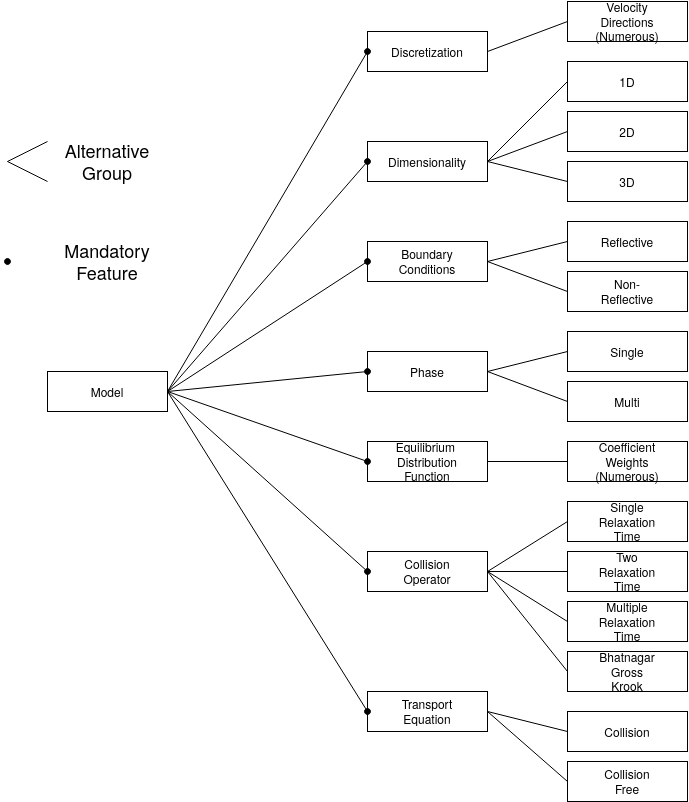
\includegraphics[width=0.5\textwidth]{FeatureDiagramLBS}
		\caption{LBS Model Feature Diagram}
		\label{LBSFeatureDiagram}
	\end{center}
\end{figure} 

\subsection{Commonalities}\label{comm_sec}

This section lists common features among potential family members. The commonalities are organized using the following abstraction of the system, which can be used to describe all Lattice Boltzmann systems: input information, generate the simulation, output the results. Section \ref{comm_lbm} describes the commonalities for the simulation step. Section \ref{comm_in} highlights the input information that is required for Lattice Boltzmann systems. The next section, Section \ref{comm_out}, shows the common features for the output of Lattice Boltzmann systems, such as the requirement that mesh information be written to files. Although the output information could simply be written to the computer’s memory, in all practical applications it is desirable to have a persistent record of the output that was created. The final section covers qualities of the system that cannot be classified as input, simulation generation or output. These commonalities are termed nonfunctional requirements of the system. For instance, all systems will have the goal that the response time to a user’s request is small enough to allow the user to focus on his/her problem and to maintain his/her train of thought, without being distracted by excessive waiting time. The commonality in this case is refined by a later variability because the specific requirement on the response time will depend on the intended usage of the mesh generating system. 

Each commonality below uses the same structure. All of the commonalities are assigned a unique item number, which takes the form of a natural number with the prefix ``C''. Following this, a description of the commonality is provided along with a list of related variabilities, which are given as hyperlinks that allow navigation of the document to the text describing the variability.  

\subsubsection{Lattice Boltzmann Method Solvers}\label{comm_lbm}
\noindent
\begin{minipage}{\textwidth}
	\renewcommand*{\arraystretch}{1.5}
	\begin{tabular}{| p{\colAwidth} | p{\colBwidth}|}
		\hline
		\bf Item Number& C\refstepcounter{comnum}\thecomnum{}\label{lattice} \\
		\hline
	\end{tabular}\\
	
	\begin{tabular}{| p{\colAwidth} | p{\colBwidth}|}		
		\hline
		\bf Description & A lattice discretizes a computational domain into a finite number of points. All LBS discretize the computational domain using a regular, evenly spaced grid within a boundary.\\
		\hline
		\bf Related Variability & \vref{numveldir} \vref{varcolop} \vref{varboundary}\\
		\hline
	\end{tabular}
\end{minipage}
~\newline
~\newline
\noindent
\begin{minipage}{\textwidth}
	\renewcommand*{\arraystretch}{1.5}
	\begin{tabular}{| p{\colAwidth} | p{\colBwidth}|}
		\hline
		\bf Item Number& C\refstepcounter{comnum}\thecomnum\label{collisionoperator} \\
		\hline
	\end{tabular}\\
	
	\begin{tabular}{| p{\colAwidth} | p{\colBwidth}|}		
		\hline
		\bf Description & All Lattice Boltzmann versions use a collision operator which concerns collisions between particles.\\
		\hline
		\bf Related Variability & \vref{dimensions} \vref{numveldir}\\
		\hline
	\end{tabular}
\end{minipage}
~\newline
~\newline
\noindent
\begin{minipage}{\textwidth}
	\renewcommand*{\arraystretch}{1.5}
	\begin{tabular}{| p{\colAwidth} | p{\colBwidth}|}
		\hline
		\bf Item Number& C\refstepcounter{comnum}\thecomnum\label{probabilitydensityfunc} \\
		\hline
	\end{tabular}\\
	
	\begin{tabular}{| p{\colAwidth} | p{\colBwidth}|}		
		\hline
		\bf Description & All Lattice Boltzmann versions use a probability density function to give the probability that fluid has moved into a specific domain.\\
		\hline
		\bf Related Variability & \vref{dimensions}\\
		\hline
	\end{tabular}
\end{minipage}
~\newline
~\newline
\noindent
\begin{minipage}{\textwidth}
	\renewcommand*{\arraystretch}{1.5}
	\begin{tabular}{| p{\colAwidth} | p{\colBwidth}|}
		\hline
		\bf Item Number& C\refstepcounter{comnum}\thecomnum\label{equildistfunc} \\
		\hline
	\end{tabular}\\
	
	\begin{tabular}{| p{\colAwidth} | p{\colBwidth}|}		
		\hline
		\bf Description & Every Lattice Boltzmann version uses an equilibrium distribution function to capture the probability distribution of particles.\\
		\hline
		\bf Related Variability & \vref{varedf} \vref{edfstorage} \vref{edfcoeff}\\
		\hline
	\end{tabular}
\end{minipage}
~\newline
~\newline
\noindent
\begin{minipage}{\textwidth}
	\renewcommand*{\arraystretch}{1.5}
	\begin{tabular}{| p{\colAwidth} | p{\colBwidth}|}
		\hline
		\bf Item Number& C\refstepcounter{comnum}\thecomnum\label{Boltzmanntransequ} \\
		\hline
	\end{tabular}\\
	
	\begin{tabular}{| p{\colAwidth} | p{\colBwidth}|}		
		\hline
		\bf Description & Every Lattice Boltzmann version uses a Boltzmann transport equation to describe the statistical behaviour of a system that does not have collisions.\\
		\hline
		\bf Related Variability & \vref{vartraneq}\\
		\hline
	\end{tabular}
\end{minipage}\\
\subsubsection{Input}\label{comm_in}
\noindent
\begin{minipage}{\textwidth}
	\renewcommand*{\arraystretch}{1.5}
	\begin{tabular}{| p{\colAwidth} | p{\colBwidth}|}
		\hline
		\bf Item Number& C\refstepcounter{comnum}\thecomnum\label{fluidandboundaryinfo} \\
		\hline
	\end{tabular}\\
	
	\begin{tabular}{| p{\colAwidth} | p{\colBwidth}|}		
		\hline
		\bf Description & The LBS require fluid, model, and boundary information for the problem.\\
		\hline
		\bf Related Variability & \vref{interface}\\
		\hline
	\end{tabular}
\end{minipage}\\
\subsubsection{Output}\label{comm_out}
\noindent
\begin{minipage}{\textwidth}
	\renewcommand*{\arraystretch}{1.5}
	\begin{tabular}{| p{\colAwidth} | p{\colBwidth}|}
		\hline
		\bf Item Number& C\refstepcounter{comnum}\thecomnum\label{predictionstomemory} \\
		\hline
	\end{tabular}\\
	
	\begin{tabular}{| p{\colAwidth} | p{\colBwidth}|}		
		\hline
		\bf Description & LBS write fluid parameter predictions to memory.\\
		\hline
		\bf Related Variability & \vref{varvisual} \vref{formatoutput} \\
		\hline
	\end{tabular}
\end{minipage}\\
\subsubsection{Nonfunctional Requirements}\label{comm_nfr}
\noindent
\begin{minipage}{\textwidth}
	\renewcommand*{\arraystretch}{1.5}
	\begin{tabular}{| p{\colAwidth} | p{\colBwidth}|}
		\hline
		\bf Item Number& C\refstepcounter{comnum}\thecomnum\label{precision} \\
		\hline
	\end{tabular}\\
	
	\begin{tabular}{| p{\colAwidth} | p{\colBwidth}|}		
		\hline
		\bf Description & LBS provide the precision required for the particular problems it is intended to solve.\\
		\hline
		\bf Related Variability & \vref{varprecise}\\
		\hline
	\end{tabular}
\end{minipage}
~\newline
~\newline
\noindent
\begin{minipage}{\textwidth}
	\renewcommand*{\arraystretch}{1.5}
	\begin{tabular}{| p{\colAwidth} | p{\colBwidth}|}
		\hline
		\bf Item Number& C\refstepcounter{comnum}\thecomnum\label{accuracy} \\
		\hline
	\end{tabular}\\
	
	\begin{tabular}{| p{\colAwidth} | p{\colBwidth}|}		
		\hline
		\bf Description & LBS provide the accuracy required for the particular problems it is intended to solve.\\
		\hline
		\bf Related Variability & \vref{varaccuracy}\\
		\hline
	\end{tabular}
\end{minipage}
~\newline
~\newline
\noindent
\begin{minipage}{\textwidth}
	\renewcommand*{\arraystretch}{1.5}
	\begin{tabular}{| p{\colAwidth} | p{\colBwidth}|}
		\hline
		\bf Item Number& C\refstepcounter{comnum}\thecomnum\label{performance} \\
		\hline
	\end{tabular}\\
	
	\begin{tabular}{| p{\colAwidth} | p{\colBwidth}|}		
		\hline
		\bf Description & The response time is small enough to allow the user to focus on their problem without being distracted by excessive waiting times.\\
		\hline
		\bf Related Variability & \vref{varresponsetime}\\
		\hline
	\end{tabular}
\end{minipage}
~\newline
~\newline
\noindent
\begin{minipage}{\textwidth}
	\renewcommand*{\arraystretch}{1.5}
	\begin{tabular}{| p{\colAwidth} | p{\colBwidth}|}
		\hline
		\bf Item Number& C\refstepcounter{comnum}\thecomnum\label{portability} \\
		\hline
	\end{tabular}\\
	
	\begin{tabular}{| p{\colAwidth} | p{\colBwidth}|}		
		\hline
		\bf Description & LBS will be as portable to other operating systems as required by the users.\\
		\hline
		\bf Related Variability & \vref{varportability}\\
		\hline
	\end{tabular}
\end{minipage}
~\newline
~\newline
\noindent
\begin{minipage}{\textwidth}
	\renewcommand*{\arraystretch}{1.5}
	\begin{tabular}{| p{\colAwidth} | p{\colBwidth}|}
		\hline
		\bf Item Number& C\refstepcounter{comnum}\thecomnum\label{usability} \\
		\hline
	\end{tabular}\\
	
	\begin{tabular}{| p{\colAwidth} | p{\colBwidth}|}		
		\hline
		\bf Description & The use of LBS is easy and efficient.\\
		\hline
		\bf Related Variability & \vref{varusability}\\
		\hline
	\end{tabular}
\end{minipage}\\

\subsection{Variabilities}\label{var_sec}
This section provides a list of characteristics that may vary among family members. As in Section \ref{comm_sec}, the first three subsections on variabilities are organized into the following sublists: Mesh Generation, Input and Output. The final two subsections list variabilities that can be characterized as system constraints and as nonfunctional requirements. 

As for the commonalities, each variability is labelled with a unique item number. In this case the numbers are prepended with the letter ``V''. The other three headings provided for each variability are: Description, Related Commonality, and Related Parameter. The related commonalities and parameters are given as a set of identifiers that respectively refer back to the previous section on commonalities or refer forward to the next section on parameters of variation.

\subsubsection{Lattice Boltzmann Method Solvers}
\noindent
\begin{minipage}{\textwidth}
	\renewcommand*{\arraystretch}{1.5}
	\begin{tabular}{| p{\colCwidth} | p{\colDwidth}|}
		\hline
		\bf Item Number& V\refstepcounter{varnum}\thevarnum\label{parallel} \\
		\hline
	\end{tabular}\\
	
	\begin{tabular}{| p{\colCwidth} | p{\colDwidth}|}		
		\hline
		\bf Description & LBS may use a framework for parallel processing of the model.\\
		\hline
		\bf Related Commonality & None\\
		\hline
		\bf Related Parameter & \pref{parparallel}\\
		\hline
	\end{tabular}
\end{minipage}\\
~\newline\\
\begin{minipage}{\textwidth}
	\renewcommand*{\arraystretch}{1.5}
	\begin{tabular}{| p{\colCwidth} | p{\colDwidth}|}
		\hline
		\bf Item Number& V\refstepcounter{varnum}\thevarnum\label{varedf} \\
		\hline
	\end{tabular}\\
	
	\begin{tabular}{| p{\colCwidth} | p{\colDwidth}|}		
		\hline
		\bf Description & Different versions of an equilibrium distribution function can capture the probability distribution of particles.\\
		\hline
		\bf Related Commonality & \cref{equildistfunc}\\
		\hline
		\bf Related Parameter & \pref{paredf}\\
		\hline
	\end{tabular}
\end{minipage}
~\newline
~\newline
\noindent
\begin{minipage}{\textwidth}
	\renewcommand*{\arraystretch}{1.5}
	\begin{tabular}{| p{\colCwidth} | p{\colDwidth}|}
		\hline
		\bf Item Number& V\refstepcounter{varnum}\thevarnum\label{edfstorage} \\
		\hline
	\end{tabular}\\
	
	\begin{tabular}{| p{\colCwidth} | p{\colDwidth}|}		
		\hline
		\bf Description & Storage patters for distribution function can vary.\\
		\hline
		\bf Related Commonality & \cref{equildistfunc}\\
		\hline
		\bf Related Parameter & \pref{parstorage}\\
		\hline
	\end{tabular}
\end{minipage}
~\newline
~\newline
\noindent
\begin{minipage}{\textwidth}
	\renewcommand*{\arraystretch}{1.5}
	\begin{tabular}{| p{\colCwidth} | p{\colDwidth}|}
		\hline
		\bf Item Number& V\refstepcounter{varnum}\thevarnum\label{edfcoeff} \\
		\hline
	\end{tabular}\\
	
	\begin{tabular}{| p{\colCwidth} | p{\colDwidth}|}		
		\hline
		\bf Description & Coefficients for distribution function can vary.\\
		\hline
		\bf Related Commonality & \cref{equildistfunc}\\
		\hline
		\bf Related Parameter & \pref{paredfcoeff}\\
		\hline
	\end{tabular}
\end{minipage}
~\newline
~\newline
\noindent
\begin{minipage}{\textwidth}
	\renewcommand*{\arraystretch}{1.5}
	\begin{tabular}{| p{\colCwidth} | p{\colDwidth}|}
		\hline
		\bf Item Number& V\refstepcounter{varnum}\thevarnum\label{dimensions} \\
		\hline
	\end{tabular}\\
	
	\begin{tabular}{| p{\colCwidth} | p{\colDwidth}|}		
		\hline
		\bf Description & The number of dimensions in the lattice of the model can vary.\\
		\hline
		\bf Related Commonality & \cref{lattice} \cref{probabilitydensityfunc}\\
		\hline
		\bf Related Parameter & \pref{pardimensions}\\
		\hline
	\end{tabular}
\end{minipage}
~\newline
~\newline
\noindent
\begin{minipage}{\textwidth}
	\renewcommand*{\arraystretch}{1.5}
	\begin{tabular}{| p{\colCwidth} | p{\colDwidth}|}
		\hline
		\bf Item Number& V\refstepcounter{varnum}\thevarnum\label{numveldir} \\
		\hline
	\end{tabular}\\
	
	\begin{tabular}{| p{\colCwidth} | p{\colDwidth}|}		
		\hline 
		\bf Description & The number of velocity directions in the lattice of the model can vary.\\
		\hline
		\bf Related Commonality & \cref{lattice} \cref{collisionoperator}\\
		\hline
		\bf Related Parameter & \pref{parveldir}\\
		\hline
	\end{tabular}
\end{minipage}
~\newline
~\newline
\noindent
\begin{minipage}{\textwidth}
	\renewcommand*{\arraystretch}{1.5}
	\begin{tabular}{| p{\colCwidth} | p{\colDwidth}|}
		\hline
		\bf Item Number& V\refstepcounter{varnum}\thevarnum\label{varcolop} \\
		\hline
	\end{tabular}\\
	
	\begin{tabular}{| p{\colCwidth} | p{\colDwidth}|}		
		\hline
		\bf Description & Various collision operators can be used.\\
		\hline
		\bf Related Commonality & \cref{lattice} \cref{collisionoperator}\\
		\hline
		\bf Related Parameter & \pref{parcollisop}\\
		\hline
	\end{tabular}
\end{minipage}
~\newline
~\newline
\noindent
\begin{minipage}{\textwidth}
	\renewcommand*{\arraystretch}{1.5}
	\begin{tabular}{| p{\colCwidth} | p{\colDwidth}|}
		\hline
		\bf Item Number& V\refstepcounter{varnum}\thevarnum\label{vartraneq} \\
		\hline
	\end{tabular}\\
	
	\begin{tabular}{| p{\colCwidth} | p{\colDwidth}|}		
		\hline
		\bf Description & Various transport equations can be used to describe the statistical behaviour of the system\\
		\hline
		\bf Related Commonality & \cref{Boltzmanntransequ}\\
		\hline
		\bf Related Parameter & \pref{partransequ}\\
		\hline
	\end{tabular}
\end{minipage}
~\newline
~\newline
\noindent
\begin{minipage}{\textwidth}
	\renewcommand*{\arraystretch}{1.5}
	\begin{tabular}{| p{\colCwidth} | p{\colDwidth}|}
		\hline
		\bf Item Number&  V\refstepcounter{varnum}\thevarnum\label{numberoffluids} \\
		\hline
	\end{tabular}\\
	
	\begin{tabular}{| p{\colCwidth} | p{\colDwidth}|}		
		\hline
		\bf Description & The number of fluids allowed in the LBS.\\
		\hline
		\bf Related Commonality & \cref{fluidandboundaryinfo}\\
		\hline
		\bf Related Parameter & \pref{parfluids}\\
		\hline
	\end{tabular}
\end{minipage}
~\newline
~\newline
\noindent
\begin{minipage}{\textwidth}
	\renewcommand*{\arraystretch}{1.5}
	\begin{tabular}{| p{\colCwidth} | p{\colDwidth}|}
		\hline
		\bf Item Number&  V\refstepcounter{varnum}\thevarnum\label{typefluidparm} \\
		\hline
	\end{tabular}\\
	
	\begin{tabular}{| p{\colCwidth} | p{\colDwidth}|}		
		\hline
		\bf Description & The type of fluid parameters.\\
		\hline
		\bf Related Commonality & \cref{fluidandboundaryinfo}\\
		\hline
		\bf Related Parameter & \pref{partypeparm}\\
		\hline
	\end{tabular}
\end{minipage}
~\newline
~\newline
\noindent
\begin{minipage}{\textwidth}
	\renewcommand*{\arraystretch}{1.5}
	\begin{tabular}{| p{\colCwidth} | p{\colDwidth}|}
		\hline
		\bf Item Number&  V\refstepcounter{varnum}\thevarnum\label{varboundary} \\
		\hline
	\end{tabular}\\
	
	\begin{tabular}{| p{\colCwidth} | p{\colDwidth}|}		
		\hline
		\bf Description & The boundary of the lattice can have various conditions.\\
		\hline
		\bf Related Commonality & \cref{lattice}\\
		\hline
		\bf Related Parameter & \pref{parboundary}\\
		\hline
	\end{tabular}
\end{minipage}\\
\subsubsection{Input}
\noindent
\begin{minipage}{\textwidth}
	\renewcommand*{\arraystretch}{1.5}
	\begin{tabular}{| p{\colCwidth} | p{\colDwidth}|}
		\hline
		\bf Item Number& V\refstepcounter{varnum}\thevarnum\label{interface} \\
		\hline
	\end{tabular}\\
	
	\begin{tabular}{| p{\colCwidth} | p{\colDwidth}|}		
		\hline
		\bf Description & The input interface can vary between LBS.\\
		\hline
		\bf Related Commonality & \cref{fluidandboundaryinfo}\\
		\hline
		\bf Related Parameter & \pref{parinterface}\\
		\hline
	\end{tabular}
\end{minipage}\\
\subsubsection{Output}
\noindent
\begin{minipage}{\textwidth}
	\renewcommand*{\arraystretch}{1.5}
	\begin{tabular}{| p{\colCwidth} | p{\colDwidth}|}
		\hline
		\bf Item Number& V\refstepcounter{varnum}\thevarnum\label{varvisual} \\
		\hline
	\end{tabular}\\
	
	\begin{tabular}{| p{\colCwidth} | p{\colDwidth}|}		
		\hline
		\bf Description & Visual presentation of the prediction.\\
		\hline
		\bf Related Commonality & \cref{predictionstomemory}\\
		\hline
		\bf Related Parameter & \pref{parvarvisual}\\
		\hline
	\end{tabular}
\end{minipage}
~\newline
~\newline
\noindent
\begin{minipage}{\textwidth}
	\renewcommand*{\arraystretch}{1.5}
	\begin{tabular}{| p{\colCwidth} | p{\colDwidth}|}
		\hline
		\bf Item Number& V\refstepcounter{varnum}\thevarnum\label{formatoutput} \\
		\hline
	\end{tabular}\\
	
	\begin{tabular}{| p{\colCwidth} | p{\colDwidth}|}		
		\hline
		\bf Description & Format of prediction information.\\
		\hline
		\bf Related Commonality & \cref{predictionstomemory}\\
		\hline
		\bf Related Parameter & \pref{parformatoutput}\\
		\hline
	\end{tabular}
\end{minipage}\\
\subsubsection{System Constraints}
\noindent
\begin{minipage}{\textwidth}
	\renewcommand*{\arraystretch}{1.5}
	\begin{tabular}{| p{\colCwidth} | p{\colDwidth}|}
		\hline
		\bf Item Number& V\refstepcounter{varnum}\thevarnum\label{processing} \\
		\hline
	\end{tabular}\\
	
	\begin{tabular}{| p{\colCwidth} | p{\colDwidth}|}		
		\hline
		\bf Description & Hardware that processes the calculations\\
		\hline
		\bf Related Commonality & None \\
		\hline
		\bf Related Parameter & \pref{parprocessing}\\
		\hline
	\end{tabular}
\end{minipage}
~\newline
~\newline
\noindent
\begin{minipage}{\textwidth}
	\renewcommand*{\arraystretch}{1.5}
	\begin{tabular}{| p{\colCwidth} | p{\colDwidth}|}
		\hline
		\bf Item Number& V\refstepcounter{varnum}\thevarnum\label{operatingsystem} \\
		\hline
	\end{tabular}\\
	
	\begin{tabular}{| p{\colCwidth} | p{\colDwidth}|}		
		\hline
		\bf Description & Operating systems on which LBS run.\\
		\hline
		\bf Related Commonality & None \\
		\hline
		\bf Related Parameter & \pref{paropsystem}\\
		\hline
	\end{tabular}
\end{minipage}
~\newline
~\newline
\noindent
\begin{minipage}{\textwidth}
	\renewcommand*{\arraystretch}{1.5}
	\begin{tabular}{| p{\colCwidth} | p{\colDwidth}|}
		\hline
		\bf Item Number& V\refstepcounter{varnum}\thevarnum\label{storage} \\
		\hline
	\end{tabular}\\
	
	\begin{tabular}{| p{\colCwidth} | p{\colDwidth}|}		
		\hline
		\bf Description & Amount of storage and memory needed for the LBS.\\
		\hline
		\bf Related Commonality & None \\
		\hline
		\bf Related Parameter & \pref{parstorageconst}\\
		\hline
	\end{tabular}
\end{minipage}\\
\subsubsection{Nonfunctional Requirements}
\noindent
\begin{minipage}{\textwidth}
	\renewcommand*{\arraystretch}{1.5}
	\begin{tabular}{| p{\colCwidth} | p{\colDwidth}|}
		\hline
		\bf Item Number& V\refstepcounter{varnum}\thevarnum\label{varprecise} \\
		\hline
	\end{tabular}\\
	
	\begin{tabular}{| p{\colCwidth} | p{\colDwidth}|}		
		\hline
		\bf Description & The precision needed for each input and output.\\
		\hline
		\bf Related Commonality & \cref{precision}\\
		\hline
		\bf Related Parameter & \pref{parprecise}\\
		\hline
	\end{tabular}
\end{minipage}
~\newline
~\newline
\noindent
\begin{minipage}{\textwidth}
	\renewcommand*{\arraystretch}{1.5}
	\begin{tabular}{| p{\colCwidth} | p{\colDwidth}|}
		\hline
		\bf Item Number& V\refstepcounter{varnum}\thevarnum\label{varaccuracy} \\
		\hline
	\end{tabular}\\
	
	\begin{tabular}{| p{\colCwidth} | p{\colDwidth}|}		
		\hline
		\bf Description & The required accuracy for the output.\\
		\hline
		\bf Related Commonality & \cref{accuracy}\\
		\hline
		\bf Related Parameter & \pref{paraccuracy}\\
		\hline
	\end{tabular}
\end{minipage}
~\newline
~\newline
\noindent
\begin{minipage}{\textwidth}
	\renewcommand*{\arraystretch}{1.5}
	\begin{tabular}{| p{\colCwidth} | p{\colDwidth}|}
		\hline
		\bf Item Number& V\refstepcounter{varnum}\thevarnum\label{varresponsetime} \\
		\hline
	\end{tabular}\\
	
	\begin{tabular}{| p{\colCwidth} | p{\colDwidth}|}		
		\hline
		\bf Description & The response time required for user interaction with the system varies.\\
		\hline
		\bf Related Commonality & \cref{performance}\\
		\hline
		\bf Related Parameter & \pref{parresponse}\\
		\hline
	\end{tabular}
\end{minipage}
~\newline
~\newline
\noindent
\begin{minipage}{\textwidth}
	\renewcommand*{\arraystretch}{1.5}
	\begin{tabular}{| p{\colCwidth} | p{\colDwidth}|}
		\hline
		\bf Item Number& V\refstepcounter{varnum}\thevarnum\label{varportability} \\
		\hline
	\end{tabular}\\
	
	\begin{tabular}{| p{\colCwidth} | p{\colDwidth}|}		
		\hline
		\bf Description & The operating systems on which a LBS can run.\\
		\hline
		\bf Related Commonality & \cref{portability}\\
		\hline
		\bf Related Parameter & \pref{parportability}\\
		\hline
	\end{tabular}
\end{minipage}
~\newline
~\newline
\noindent
\begin{minipage}{\textwidth}
	\renewcommand*{\arraystretch}{1.5}
	\begin{tabular}{| p{\colCwidth} | p{\colDwidth}|}
		\hline
		\bf Item Number& V\refstepcounter{varnum}\thevarnum\label{varusability} \\
		\hline
	\end{tabular}\\
	
	\begin{tabular}{| p{\colCwidth} | p{\colDwidth}|}		
		\hline
		\bf Description & The ease with which LBS can effectively be run varies.\\
		\hline
		\bf Related Commonality & \cref{usability}\\
		\hline
		\bf Related Parameter & \pref{parusability}\\
		\hline
	\end{tabular}
\end{minipage}\\
\newpage
\subsection{Parameters of Variation}
This section specifies the parameters of variation for the variabilities listed in Section \ref{var_sec}. They are organized into the same five subcategories as employed previously: Mesh Generation, Input, Output, System Constraints, Nonfunctional Requirements. 

Each parameter of variation is given a unique identifier of the form “P” followed by a natural number. The corresponding variability is listed and a hyperlink is provided that allows navigation back to the appropriate item in Section \ref{var_sec}. The final entry for each parameter of variation is the binding time, which is the time in the software lifecycle when the variability is fixed. The binding time could be during specification, or during building
of the system (compile time), or during execution of the system (run time). It is possible to have a mixture of binding times. For instance, a parameter of variation could have a binding time of “specification or building” to represent that the parameter could be set at specification time, or it could be postponed until the given family member is built. The choice of postponing the decision until the build could be associated with the presence of a domain specific language that would allow postponing decisions on the values of the parameter of variation.

\subsubsection{Lattice Boltzmann Method Solvers}
\noindent
\begin{minipage}{\textwidth}
	\renewcommand*{\arraystretch}{1.5}
	\begin{tabular}{| p{\colEwidth} | p{\colFwidth}|}
		\hline
		\bf Item Number& P\refstepcounter{parnum}\theparnum\label{parparallel} \\
		\hline
	\end{tabular}\\
	
	\begin{tabular}{| p{\colEwidth} | p{\colFwidth}|}		
		\hline
		\bf Corresponding Variability & \vref{parallel}\\
		\hline
		\bf Range of Parameters & OpenMP, OpenCL, CUDA, MPI are used if the execution of the LBS is parallelized.\\
		\hline
		\bf Binding Time & Build Time\\
		\hline
	\end{tabular}
\end{minipage}
~\newline
~\newline
\noindent
\begin{minipage}{\textwidth}
	\renewcommand*{\arraystretch}{1.5}
	\begin{tabular}{| p{\colEwidth} | p{\colFwidth}|}
		\hline
		\bf Item Number& P\refstepcounter{parnum}\theparnum\label{paredf} \\
		\hline
	\end{tabular}\\
	
	\begin{tabular}{| p{\colEwidth} | p{\colFwidth}|}		
		\hline
		\bf Corresponding Variability & \vref{parallel}\\
		\hline
		\bf Range of Parameters & Equilibrium can be approximated up to different orders in incompressible or compressible versions.\\
		\hline
		\bf Binding Time & Build Time\\
		\hline
	\end{tabular}
\end{minipage}
~\newline
~\newline
\noindent
\begin{minipage}{\textwidth}
	\renewcommand*{\arraystretch}{1.5}
	\begin{tabular}{| p{\colEwidth} | p{\colFwidth}|}
		\hline
		\bf Item Number& P\refstepcounter{parnum}\theparnum\label{parstorage} \\
		\hline
	\end{tabular}\\
	
	\begin{tabular}{| p{\colEwidth} | p{\colFwidth}|}		
		\hline
		\bf Corresponding Variability & \vref{edfstorage}\\
		\hline
		\bf Range of Parameters & Single and multiple array storage patterns can be used.\\
		\hline
		\bf Binding Time & Build Time\\
		\hline
	\end{tabular}
\end{minipage}
~\newline
~\newline
\noindent
\begin{minipage}{\textwidth}
	\renewcommand*{\arraystretch}{1.5}
	\begin{tabular}{| p{\colEwidth} | p{\colFwidth}|}
		\hline
		\bf Item Number& P\refstepcounter{parnum}\theparnum\label{paredfcoeff} \\
		\hline
	\end{tabular}\\
	
	\begin{tabular}{| p{\colEwidth} | p{\colFwidth}|}		
		\hline
		\bf Corresponding Variability & \vref{edfcoeff}\\
		\hline
		\bf Range of Parameters & Numerous coefficients for equilibrium distribution function based on number of velocity directions. \\
		\hline
		\bf Binding Time & Build Time\\
		\hline
	\end{tabular}
\end{minipage}
~\newline
~\newline
\noindent
\begin{minipage}{\textwidth}
	\renewcommand*{\arraystretch}{1.5}
	\begin{tabular}{| p{\colEwidth} | p{\colFwidth}|}
		\hline
		\bf Item Number& P\refstepcounter{parnum}\theparnum\label{pardimensions} \\
		\hline
	\end{tabular}\\
	
	\begin{tabular}{| p{\colEwidth} | p{\colFwidth}|}		
		\hline
		\bf Corresponding Variability & \vref{dimensions}\\
		\hline
		\bf Range of Parameters & LBS models can have up to 3 dimensions.\\
		\hline
		\bf Binding Time & Build Time or Run Time\\
		\hline
	\end{tabular}
\end{minipage}
~\newline
~\newline
\noindent
\begin{minipage}{\textwidth}
	\renewcommand*{\arraystretch}{1.5}
	\begin{tabular}{| p{\colEwidth} | p{\colFwidth}|}
		\hline
		\bf Item Number& P\refstepcounter{parnum}\theparnum\label{parveldir} \\
		\hline
	\end{tabular}\\
	
	\begin{tabular}{| p{\colEwidth} | p{\colFwidth}|}		
		\hline
		\bf Corresponding Variability & \vref{numveldir}\\
		\hline
		\bf Range of Parameters & One dimensional models include options of 2, 3, and 5 velocity directions. Two dimensional models include options of 9, 13, and 15 velocity directions. Three dimensional models include options of 15, 19, and 27 velocity directions. \\
		\hline
		\bf Binding Time & Build Time or Run Time\\
		\hline
	\end{tabular}
\end{minipage}
~\newline
~\newline
\noindent
\begin{minipage}{\textwidth}
	\renewcommand*{\arraystretch}{1.5}
	\begin{tabular}{| p{\colEwidth} | p{\colFwidth}|}
		\hline
		\bf Item Number& P\refstepcounter{parnum}\theparnum\label{parcollisop} \\
		\hline
	\end{tabular}\\
	
	\begin{tabular}{| p{\colEwidth} | p{\colFwidth}|}		
		\hline
		\bf Corresponding Variability & \vref{varcolop}\\
		\hline
		\bf Range of Parameters & SRT, TRT, MRT, BGK collision operators.\\
		\hline
		\bf Binding Time & Build Time\\
		\hline
	\end{tabular}
\end{minipage}
~\newline
~\newline
\noindent
\begin{minipage}{\textwidth}
	\renewcommand*{\arraystretch}{1.5}
	\begin{tabular}{| p{\colEwidth} | p{\colFwidth}|}
		\hline
		\bf Item Number& P\refstepcounter{parnum}\theparnum\label{partransequ} \\
		\hline
	\end{tabular}\\
	
	\begin{tabular}{| p{\colEwidth} | p{\colFwidth}|}		
		\hline
		\bf Corresponding Variability & \vref{vartraneq}\\
		\hline
		\bf Range of Parameters & Collision and collision free transport equations.\\
		\hline
		\bf Binding Time & Build Time\\
		\hline
	\end{tabular}
\end{minipage}
~\newline
~\newline
\noindent
\begin{minipage}{\textwidth}
	\renewcommand*{\arraystretch}{1.5}
	\begin{tabular}{| p{\colEwidth} | p{\colFwidth}|}
		\hline
		\bf Item Number& P\refstepcounter{parnum}\theparnum\label{parfluids} \\
		\hline
	\end{tabular}\\
	
	\begin{tabular}{| p{\colEwidth} | p{\colFwidth}|}		
		\hline
		\bf Corresponding Variability & \vref{numberoffluids}\\
		\hline
		\bf Range of Parameters & LBS can model one or more fluids.\\
		\hline
		\bf Binding Time & Build Time\\
		\hline
	\end{tabular}
\end{minipage}
~\newline
~\newline
\noindent
\begin{minipage}{\textwidth}
	\renewcommand*{\arraystretch}{1.5}
	\begin{tabular}{| p{\colEwidth} | p{\colFwidth}|}
		\hline
		\bf Item Number& P\refstepcounter{parnum}\theparnum\label{partypeparm} \\
		\hline
	\end{tabular}\\
	
	\begin{tabular}{| p{\colEwidth} | p{\colFwidth}|}		
		\hline
		\bf Corresponding Variability & \vref{typefluidparm}\\
		\hline
		\bf Range of Parameters & LBS fluid parameters include Reynolds Number, density, viscosity, time, pressure, force, direction, relaxation rate, turbulence.\\
		\hline
		\bf Binding Time & Build Time\\
		\hline
	\end{tabular}
\end{minipage}
~\newline
~\newline
\noindent
\begin{minipage}{\textwidth}
	\renewcommand*{\arraystretch}{1.5}
	\begin{tabular}{| p{\colEwidth} | p{\colFwidth}|}
		\hline
		\bf Item Number& P\refstepcounter{parnum}\theparnum\label{parboundary} \\
		\hline
	\end{tabular}\\
	
	\begin{tabular}{| p{\colEwidth} | p{\colFwidth}|}		
		\hline
		\bf Corresponding Variability & \vref{varboundary}\\
		\hline
		\bf Range of Parameters & Lattice boundary can have reflective or non-reflective conditions.\\
		\hline
		\bf Binding Time & Build Time\\
		\hline
	\end{tabular}
\end{minipage}\\
\subsubsection{Input}
\noindent
\begin{minipage}{\textwidth}
	\renewcommand*{\arraystretch}{1.5}
	\begin{tabular}{| p{\colEwidth} | p{\colFwidth}|}
		\hline
		\bf Item Number& P\refstepcounter{parnum}\theparnum\label{parinterface} \\
		\hline
	\end{tabular}\\
	
	\begin{tabular}{| p{\colEwidth} | p{\colFwidth}|}		
		\hline
		\bf Corresponding Variability & \vref{interface}\\
		\hline
		\bf Range of Parameters & Input can be graphical, text or file.\\
		\hline
		\bf Binding Time & Build Time\\
		\hline
	\end{tabular}
\end{minipage}\\
\subsubsection{Output}
\noindent
\begin{minipage}{\textwidth}
	\renewcommand*{\arraystretch}{1.5}
	\begin{tabular}{| p{\colEwidth} | p{\colFwidth}|}
		\hline
		\bf Item Number& P\refstepcounter{parnum}\theparnum\label{parvarvisual} \\
		\hline
	\end{tabular}\\
	
	\begin{tabular}{| p{\colEwidth} | p{\colFwidth}|}		
		\hline
		\bf Corresponding Variability & \vref{varvisual}\\
		\hline
		\bf Range of Parameters & LBS can provide 1D, 2D, and 3D rendering of  the model.\\
		\hline
		\bf Binding Time & Build Time or Run Time\\
		\hline
	\end{tabular}
\end{minipage}
~\newline
~\newline
\noindent
\begin{minipage}{\textwidth}
	\renewcommand*{\arraystretch}{1.5}
	\begin{tabular}{| p{\colEwidth} | p{\colFwidth}|}
		\hline
		\bf Item Number& P\refstepcounter{parnum}\theparnum\label{parformatoutput} \\
		\hline
	\end{tabular}\\
	
	\begin{tabular}{| p{\colEwidth} | p{\colFwidth}|}		
		\hline
		\bf Corresponding Variability & \vref{formatoutput}\\
		\hline
		\bf Range of Parameters & LBS prediction information is output in either text or binary format.\\
		\hline
		\bf Binding Time & Build Time\\
		\hline
	\end{tabular}
\end{minipage}\\
\subsubsection{System Constraints}
\noindent
\begin{minipage}{\textwidth}
	\renewcommand*{\arraystretch}{1.5}
	\begin{tabular}{| p{\colEwidth} | p{\colFwidth}|}
		\hline
		\bf Item Number& P\refstepcounter{parnum}\theparnum\label{parprocessing} \\
		\hline
	\end{tabular}\\
	
	\begin{tabular}{| p{\colEwidth} | p{\colFwidth}|}		
		\hline
		\bf Corresponding Variability & \vref{processing}\\
		\hline
		\bf Range of Parameters & The LBS model can be calculated on the CPU or GPU.\\
		\hline
		\bf Binding Time & Build Time\\
		\hline
	\end{tabular}
\end{minipage}
~\newline
~\newline
\noindent
\begin{minipage}{\textwidth}
	\renewcommand*{\arraystretch}{1.5}
	\begin{tabular}{| p{\colEwidth} | p{\colFwidth}|}
		\hline
		\bf Item Number& P\refstepcounter{parnum}\theparnum\label{paropsystem} \\
		\hline
	\end{tabular}\\
	
	\begin{tabular}{| p{\colEwidth} | p{\colFwidth}|}		
		\hline
		\bf Corresponding Variability & \vref{operatingsystem}\\
		\hline
		\bf Range of Parameters & LBS can be run on Windows, MacOS, or Linux versions.\\
		\hline
		\bf Binding Time & Build Time\\
		\hline
	\end{tabular}
\end{minipage}
~\newline
~\newline
\noindent
\begin{minipage}{\textwidth}
	\renewcommand*{\arraystretch}{1.5}
	\begin{tabular}{| p{\colEwidth} | p{\colFwidth}|}
		\hline
		\bf Item Number& P\refstepcounter{parnum}\theparnum\label{parstorageconst} \\
		\hline
	\end{tabular}\\
	
	\begin{tabular}{| p{\colEwidth} | p{\colFwidth}|}		
		\hline
		\bf Corresponding Variability & \vref{storage}\\
		\hline
		\bf Range of Parameters & The amount of memory and storage varies between LBS.\\
		\hline
		\bf Binding Time & Build Time\\
		\hline
	\end{tabular}
\end{minipage}\\
\subsubsection{Nonfunctional Requirements}
\noindent
\begin{minipage}{\textwidth}
	\renewcommand*{\arraystretch}{1.5}
	\begin{tabular}{| p{\colEwidth} | p{\colFwidth}|}
		\hline
		\bf Item Number& P\refstepcounter{parnum}\theparnum\label{parprecise} \\
		\hline
	\end{tabular}\\
	
	\begin{tabular}{| p{\colEwidth} | p{\colFwidth}|}		
		\hline
		\bf Corresponding Variability & \vref{varprecise}\\
		\hline
		\bf Range of Parameters & Each input and each output will have specified the precision with which the real number is stored and/or calculated.\\
		\hline
		\bf Binding Time & Build Time or Run Time\\
		\hline
	\end{tabular}
\end{minipage}
~\newline
~\newline
\noindent
\begin{minipage}{\textwidth}
	\renewcommand*{\arraystretch}{1.5}
	\begin{tabular}{| p{\colEwidth} | p{\colFwidth}|}
		\hline
		\bf Item Number& P\refstepcounter{parnum}\theparnum\label{paraccuracy} \\
		\hline
	\end{tabular}\\
	
	\begin{tabular}{| p{\colEwidth} | p{\colFwidth}|}		
		\hline
		\bf Corresponding Variability & \vref{varaccuracy}\\
		\hline
		\bf Range of Parameters & The tolerance allowed for each output produced by the system so that the system produces usable results. \\
		\hline
		\bf Binding Time & Build Time or Run Time\\
		\hline
	\end{tabular}
\end{minipage}
~\newline
~\newline
\noindent
\begin{minipage}{\textwidth}
	\renewcommand*{\arraystretch}{1.5}
	\begin{tabular}{| p{\colEwidth} | p{\colFwidth}|}
		\hline
		\bf Item Number& P\refstepcounter{parnum}\theparnum\label{parresponse} \\
		\hline
	\end{tabular}\\
	
	\begin{tabular}{| p{\colEwidth} | p{\colFwidth}|}		
		\hline
		\bf Corresponding Variability & \vref{varresponsetime}\\
		\hline
		\bf Range of Parameters & The maximum amount of time that the user is expected to wait for the system to produce a result ranges between systems and models from near instantaneous to several minutes or longer.\\
		\hline
		\bf Binding Time & Specification\\
		\hline
	\end{tabular}
\end{minipage}
~\newline
~\newline
\noindent
\begin{minipage}{\textwidth}
	\renewcommand*{\arraystretch}{1.5}
	\begin{tabular}{| p{\colEwidth} | p{\colFwidth}|}
		\hline
		\bf Item Number& P\refstepcounter{parnum}\theparnum\label{parportability} \\
		\hline
	\end{tabular}\\
	
	\begin{tabular}{| p{\colEwidth} | p{\colFwidth}|}		
		\hline
		\bf Corresponding Variability & \vref{varportability}\\
		\hline
		\bf Range of Parameters & The ease with which LBS can run on Windows, MacOS, and Linux system varies. Some LBS can run on all three, while some can run on multiple or only one operating system.\\
		\hline
		\bf Binding Time & Specification\\
		\hline
	\end{tabular}
\end{minipage}
~\newline
~\newline
\noindent
\begin{minipage}{\textwidth}
	\renewcommand*{\arraystretch}{1.5}
	\begin{tabular}{| p{\colEwidth} | p{\colFwidth}|}
		\hline
		\bf Item Number& P\refstepcounter{parnum}\theparnum\label{parusability} \\
		\hline
	\end{tabular}\\
	
	\begin{tabular}{| p{\colEwidth} | p{\colFwidth}|}		
		\hline
		\bf Corresponding Variability & \vref{varusability}\\
		\hline
		\bf Range of Parameters & Some LBS require programming skills and domain expert knowledge while some LBS can be run without such skills.\\
		\hline
		\bf Binding Time & Specification\\
		\hline
	\end{tabular}
\end{minipage}

\newpage
\section{Methodology - DONE SECTION 1st DRAFT}

In this project we set out to answer the research questions found in Section \ref{researchquestions} for the LBM SCS domain. The process involved systematically measuring and analyzing members of this software family along the quality attributes found in Section \ref{softwarequalities}. This included gathering quantitative and qualitative measurements. A goal of the project was to produce a hierarchical quality assessment for LBM software packages.  

We collected quantitative data using the measures found in the measurement template of Section \ref{measurementtemplate}. Some of this was empirical software engineering related data, such as the number of files, number of lines of code, percentage of issues that are closed. Most of the data was gathered by manually observing the software, its source code, and its artifacts, while some was gathered using the tools listed in Section \ref{tools}.

We also collected qualitative data by interviewing the software package developers and asking them the questions found in Section \ref{interviewquestions}. Furthermore, we solicited the assistance of domain experts to better assess each software package by leveraging their experience to assess the functional and non-functional requirements for the software domain. 

This section begins by describing the steps of the overall process we used to select, measure and compare LBM software. This is followed by quality definitions and how these qualities were assessed in our project. The rest of the section provides an overview of how candidate software packages were selected and filtered, the empirical measurements and software tools that were used, and the analytic hierarchy process (AHP). 

\subsection{Process}

 The following steps provide an overview of how the assessment was conducted: 

\begin{enumerate}
	\item List candidate software packages for the domain. This is discussed in Section \ref{identifysoftware}.
	\item Filter the software package list. This is discussed in Section \ref{filtersoftware}.
	\item Gather the source code and documentation for each software package.
	\item Collect empirical measures. This is discussed in Section \ref{empiricalmeasures}.
	\item Measure using the measurement template. This is discussed in Section \ref{empiricalmeasures}. The measurement template can be found in Section \ref{measurementtemplate2}.
	\item Survey the developers. The developers of each software package in the filtered software list were contacted for voluntary interviews. Four interviews were conducted in total. The interview questions can be found in Section \ref{interviewquestions}.
	\item Use AHP to rank the software packages. This is discussed in Section \ref{AHP}.
	\item Analyze the results and answer the research questions. The answers can be found in section \ref{answersquestions}.
\end{enumerate}

These steps are further detailed in the Methodology for Assessing the State of the Practice for Domain X document found \href{https://github.com/smiths/AIMSS/blob/master/StateOfPractice/Methodology/Methodology.pdf}{here}. 

\subsection{Software Qualities}\label{softwarequalities}

Software quality attributes facilitate the measurement and comparison of software packages in this state of the practice assessment. In this report we adopt software quality definitions from various researchers and subject matter expert entities. Some of the definitions are from \cite{Smithetal2020}. The quality measurement results are found in Section \ref{qualityresults} of this report. Section \ref{qualityrecommentations} lists recommendations to address software qualities in LBM software packages. The following are the software quality definitions used in this state of the practice exercise, along with comments regarding their quantitative and qualitative measurement.

\subsubsection{Installability} 

Installability is measured by the effort required for the installation, uninstallation or reinstallation of a software product in a specified
environment \citep{ISO/IEC25010} \citep{lenhard2013measuring}. A good measure of installability correlates with scenarios when low or moderate effort is required to gather and prepare software for its general use on a system for which it was designed. In this case effort includes the time spent finding and understanding the installation instructions, the man-time and resources spent performing the installation procedure, and the absence or ease of overcoming system compatibility issues. The ability to reasonably validate the installation procedure also has a positive effect on the measure of installability. Similarly, the ease of uninstallation has an affect on the measure of installability. 

\subsubsection{Correctness}

 A software program is correct if it behaves according to its stated
specifications \citep{GhezziEtAl2003}. This requires that the specification is available. Software is less likely to have a formal specification if it is not developed by seasoned or professional software developers. Since some software does not have a specification available, the correctness of software cannot always be verified. Despite an absent specification, the correctness of the output of scientific computing software can sometimes be manually verified by applying domain knowledge. A good measure of correctness correlates with the availability of a requirements specification and reference to domain theory, as well as the explicit use of tools or techniques for building confidence of correctness, such as documentation generators and software analysis tools.

\subsubsection{Verifiability}

Verifiability is measured by the extent to which a set of tests can be written and executed to demonstrate that the delivered system meets the specification \citep{sommerville}. Similarly to correctness, verifiability is correlated with the availability of a specification and with reference to domain knowledge. A good measure of verifiability is further correlated with the availability of well written tutorials that include expected output, with software unit testing documentation, and with evidence of continuous integration during the development process. 

\subsubsection{Reliability}

Reliability is measured by the probability of failure-free operation of a computer program in a specified environment for a specified time, i.e. the average time interval between two failures also known as the mean time to failure (MTTF) \citep{GhezziEtAl2003} \citep{musa1987software}. Reliability is thus positively correlated with the absence of errors during installation and use. Recoverability from errors also improves reliability. In turn the presence of descriptive error messages and logs increases the ability to recover the system.

\subsubsection{Robustness}

Software possesses the characteristic of robustness if it behaves “reasonably” in two situations: i) when it encounters circumstances not anticipated in the requirements specification; and ii) when the assumptions in its requirements specification are violated \citep{boehm2007software} \citep{ghezzi1991fundamentals}. A good measure of robustness correlates with a reasonable reaction to unexpected input, including data of the wrong type, empty input, or missing files or links. A reasonable reaction includes an appropriate error message and the ability to recover the system.

\subsubsection{Performance}

Performance is measured by the degree to which a system or component accomplishes its designated functions within given constraints, such as speed (database response times, for instance), throughput (transactions per second), capacity (concurrent usage loads), and timing (hard real-time demands) \citep{IEEEStdGlossarySET1990} \citep{wiegers2003softreq}. In this state of the practice assessment performance was not quantitatively measured. Instead the documentation of each software package was observed for information that alludes to a consideration of performance, such as parallelization tools. 

\subsubsection{Usability}

Usability is measured by the extent to which a software product can be used by specified users to achieve specified goals with effectiveness, efficiency, and satisfaction in a specified context of use \citep{nielsonusability}. A good measure of usability correlates with the presence of documentation, including tutorials, manuals, and defined user characteristics, and user support. Preferably the user support model has avenues to contact developers and report issues.

\subsubsection{Maintainability}

A measure of maintainability is the effort with which a software
system or component can be modified to correct faults, improve performance or other attributes, and satisfy new requirements \citep{IEEEStdGlossarySET1990} \citep{boehm2007software}. In this state of the practice analysis maintainability is measured by the quality of documentation artifacts, and the presence of version control and issue tracking. These artifacts can greatly decrease the effort needed to modify software. There are many documentation artifacts that can improve maintainability, including user and developer manuals, specifications, README files, change logs, release notes, publications, forums, and instructional websites. 

\subsubsection{Modifiability}

Modifiability refers to the ease with which stable changes can be made to a system and the flexibility of the system to adopt such changes \citep{8016712}.
This state of the practice assessment did not quantitatively measure modifiability. Developers were asked in interviews if they considered the ease of future changes when developing the software packages, specifically changes to the structure of the system, modules and code blocks. A follow up question asked if any measures had been taken.

\subsubsection{Reusability}

Reusability refers to the extent to which components of a software package can be used with or without adaptation in other software packages \citep{kalagiakos2003non}. A good measure of reusability results from a large number of easily reusable components. Increased software modularization, defined as the presence of smaller components with well defined interfaces, is important. For this state of the practice assessment, a good measure of reusablity correlates with an increased number of code files, and the availability of API documentation.

\subsubsection{Understandability}

Understandability is measured by the capability of the software package to enable the user to understand its suitability and function \citep{ISO9126}.
It is an artifact-dependent quality. Understandability is different for the user-interface, source code, documentation. In this state of the practice analysis understandability focuses on the source code. It is measured by the consistency of a formatting style, the extend of modularization, the explicit identification of coding standards, the presence of meaningful identifiers, and clarity of comments. 

\subsubsection{Traceability}

Traceability refers to the ability to link the software implementation and the software artifacts, especially the requirement specification \citep{McCallEtAl1977}. Similar to the quality of correctness, this requires some form of specification to be available. The quality refers to keeping track of information as it changes forms or relates between artifacts. This state of the practice assessment did not quantitatively measure traceability. Developers were asked in interviews how documentation fits into their development process.

\subsubsection{Visibility and Transparency}

Visibility and transparency refer to the extent to which all of the steps of a software development process, and the current status of it, are conveyed clearly \citep{ghezzi1991fundamentals}. In this state of the practice assessment a good measure of visibility and transparency correlates with a well defined development process, the presence of development process and environment documentation, and software package version release notes. 

\subsubsection{Reproducibility}

Software achieves reproducibility if another developer can take the requirements documentation and re-obtain the same software artifacts \citep{BenureauAndRougier2017}. In this context, reproducibility refers to the similarity between artifacts. Reproducibility can also refer to the output of the software, irrespective of the artifacts, where the scientific results are compared between software implementations, or between software implementations and manually calculated results. This state of the practice assessment did not quantitatively measure reproducibility. Developers were asked in interviews if they have any concern that their computational results won’t be reproducible in the future, and if they have taken any steps to ensure reproducibility.

\subsubsection{Unambiguity}

Unambiguity refers to the extent to which two readers have similar interpretations when reading software artifacts. In other words, artifacts are unambiguous if, and only if, they only have one interpretation \citep{IEEE1998}. This state of the practice assessment did not quantitatively measure unambiguity. Developers were asked in interviews if they think that the current documentation can clearly convey all necessary knowledge to the users, and how they achieved this or what improvements are needed ot achieve it.

\subsection{Identify Candidate Software}\label{identifysoftware}

The candidate software was found through search engine queries targeting authoritative lists of software. We found LBM software listed on the websites GitHub and swMATH, as well as through articles found in scholarly journals and databases. 

The following properties were considered when creating the list and reviewing the candidate software:

\begin{enumerate}
	\item The software functionality must fall within the identified domain.
	\item The source code must be viewable.
	\item The empirical measures should be available, which implies a preference for GitHub-style repositories.
	\item The software cannot be marked as incomplete or in an initial development phase.
\end{enumerate}

The initial list had 46 packages, including a few packages that were later found to not have publicly available source code, or to be in an incomplete state of development. 

\subsection{Filter the Software List}\label{filtersoftware}

In order to reduce the number of members in the candidate software list, the following filters were applied. The filters were applied in the priority order listed.

\begin{enumerate}
	\item Scope: Software is removed by narrowing what functionality is considered to be within the scope of the domain.
	\item Usage: Software packages were eliminated if their installation procedure was missing or not clear and easy to follow.
	\item Age: The older software packages (age being measured by the last date when a change was made) were eliminated, except in the cases where an older software package appears to be highly recommended and currently in use. 
\end{enumerate}

For the third item in the above filter, software packages were characterized as `alive' if their related documentation had been updated within
the last 18 month. Packages were categorized as `dead' if the last update of this information was more than 18 month ago.\\ 

\begin{center}
	\begin{tabular}{ p{4cm}p{3cm}p{3cm} }
		\hline
		Name & Released & Updated\\
		\hline
		DL\_MESO (LBE) & unclear & 2020 Mar\\
		waLBerla & 2008 Aug & 2020 Jul\\
		Sailfish & 2012 Nov & 2019 Jun\\
		Palabos & unclear & 2020 Jul\\
		OpenLB & 2007 Jul & 2019 Oct\\
		MechSys   & 2008 Jun    & 2020 Jul\\
		LUMA&   2016 Nov   & 2020 Feb\\
		Ludwig& 2018 Aug & 2020 Jul\\
		lettuce    & 2019 May & 2020 Jul\\
		pyLBM & 2015 Jun&   2020 Jun\\
		lbmpy& unknown  & 2020 Jun  \\
		TCLB & 2013 Jun  & 2020 Apr\\
		ESPResSo & 2010 Nov & 2020 Jun\\
		ESPResSo++ & 2011 Feb & 2020 Apr\\
		\hline
	\end{tabular}
	\captionof{table}{Alive Software Packages}\label{alivepackages}
\end{center}

While the initial list had 46 packages, filtering by scope, usage, and age decreased the size of the list to 23 packages. Many of the 23 packages that were removed could not be tested as there was no installation guide, they were incomplete, source code was not publicly available, a license was needed, or the project was out of scope or not up to a standard that would support incorporating them into this study. Of the remaining 23 packages that were studied, some were kept on the list despite being marked as dead due to their prevalence on authoritative lists on LBM software and due to their surface excellence, specifically the considerable time that was put into these projects.  
The final list of software packages that were analyzed in this project can be found in the following two tables. Table \ref{alivepackages} lists packages that fell into the `alive' category as of mid 2020, and Table \ref{deadpackages} lists packages that were `dead' at that time. \\

\begin{center}
	\begin{tabular}{ p{4cm}p{3cm}p{3cm} }
		\hline
		Name & Released & Updated\\
		\hline
		SunlightLB & 2005 Sep & 2012 Nov\\
		MP-LABS & 2008 Jun & 2014 Oct\\
		LIMBES & 2010 Nov & 2014 Dec\\
		LB3D & unclear & 2012 Mar\\
		LB3D-Prime & 2005 & 2011 Oct\\
		LB2D-Prime & 2005 & 2012 Apr\\
		LatBo.jl & 2014 Aug & 2017 Feb\\
		HemeLB & 2007 Jun & 2018 Aug\\
		laboetie & 2014 Nov & 2018 Aug\\
		\hline
	\end{tabular}
	\captionof{table}{Dead Software Packages}\label{deadpackages}
\end{center}

There is considerable variation among these software packages, including their intended purpose, size, user interfaces, and software languages used. For example, the OpenLB software package is predominantly a C++ package that makes use of hybrid parallelization and was designed to address a range of computational fluid dynamics problems \citep{heuveline2009towards}. The software package pyLBM is an all-in-one Python language package for numerical simulations \citep{graille2017pylbm}. ESPResSo is an extensible simulation package that is specifically for research on soft matter, and is written in C++ and Python \citep{weik2019espresso}. The HemeLB package is used for efficient simulation of fluid flow in several medical domains, and is written predominantly in C, C++, and Python \citep{mazzeo2008hemelb}. 

\subsection{Empirical Measures}\label{empiricalmeasures}

The quality measurements in this assessment rely on the gathering and analyzing of raw and processed empirical data related to the research questions listed in Section \ref{researchquestions}. 

All of the quality measurements that are part of the AHP analysis are in this category, while qualitative data gathered during interviews with developers is not. This part of the assessment focuses on data that is reasonably easy to collect. Much of the data was gathered by manually reviewing the artifacts of each software package, while some was gathered using freeware tools listed in Section \ref{tools}. The data that was gathered is listed in the measurement template found in Section \ref{measurementtemplate2}. Some of the data required processing other data within the template, including the status of the software package which relied on the last commit date, the percentage of issues that are closed which relied on the number of open and closed issues, and the percentage of code that is comments which relied on the number of total lines and comment lines in text-based files. The complete measurement template data was then analyzed using the grading template found in Section \ref{gradingtemplate2}, the output of which was analyzed using the AHP described in Section \ref{AHP}.

\subsubsection{Software Tools}\label{tools}

Most of the measurement template data was gathered by observing GitHub repository metrics and software package artifacts, or by processing data gathered using freeware tools. Data in the final three sets of the measurement template was collected using these tools. The tool \href{https://github.com/tomgi/git_stats}{GitStats} was used to measure each software package's GitHub repository for the number of binary files, the number of added and deleted lines, and the number of commits over varying time intervals. The tool \href{https://github.com/boyter/scc}{Sloc Cloc and Code (scc)} was used to measure the number of text based files as well as the number of total, code, comment, and blank lines in each GitHub repository. Details on installing and running these tools can be found in the \href{https://github.com/smiths/AIMSS/blob/master/StateOfPractice/Methodology/A
	Guide to Empirical Measures.pdf} {Guide to Empirical Measures} file in the AIMSS repository. 

\subsection{Analytical Hierarchy Process}\label{AHP}

The Analytical Hierarchy Process (AHP) is a decision-making technique that is used to compare multiple options by multiple criteria. In our work AHP was used for comparing and ranking the LBM software packages using the overall impression quality scores that were gathered in the measurement template found in Section \ref{measurementtemplate2} using the grading template found in Section \ref{gradingtemplate2}. AHP performs a pairwise analysis using a matrix and generates an overall score as well as individual quality scores for each software package. \cite{SmithEtAl2016} shows how AHP is applied to ranking software based on quality measures. 

This project used a tool for conducting this process. The tool includes a sensitivity analysis that was used to ensure that the software package rankings are appropriate with respect to the uncertainty of the quality scores. The README file of the tool, which includes requirements and usage information, is found \href{https://github.com/smiths/AIMSS/blob/master/StateOfPractice/AHP2020/LBM/README.txt}{here}. 

\newpage
\section{Results - DONE SECTION 1st DRAFT}\label{qualityresults}

This section presents the AHP results for qualities that were quantitatively measured. Qualitiative data from interviews with some developers is also found in this section. Working quality definitions are found in section \ref{softwarequalities}.

\subsection{Installability}

All of the software packages that were tested have installation instructions. As noted previously, many of the 23 software packages removed from the original list of 46 software packages are missing documentation, including installation instructions. 

All 23 packages can be installed on some Unix-like systems. Seven packages could be installed on Windows, and 5 on macOS. Operating system compatibility is found in the documentation of 19 software packages. For this state of the practice assessment, all but one of the software packages were tested on Ubuntu. The remaining package was tested on CentOS.

Of the software packages that were tested, most installation instructions are located in one place, often in an instruction manual or on a web page. Sometimes incomplete installation instructions are found on a home page, with more detailed instructions located on another web page or within formal documentation. Maintainability and correctness of these instructions could be improved if they were limited to one location. 

All but two of the software packages have an automation procedure for at least part of the installation process. Most of these packages use make to automate the installation. A couple of packages use custom scripts for automation.

Errors encountered during the installation process were sometimes quickly fixed thanks to descriptive error messages. At other times, error messages were vague and difficult to troubleshoot. Fourteen software packages definitively broke during installation. A couple of packages did not provide a definitive message of the success or failure of installation. In these instances validating the installation required performing a tutorial or running a script, as described below, if they were available. The installation of most software packages could be recovered if a descriptive error message was displayed. Only three software packages that displayed a descriptive error message were not recoverable, and most of these instances were due to hardware and operating system incompatibility, such as the requirement of CUDA.

About half of the installation instructions are not written as if the person doing the installation has none of the dependent packages installed, and many software packages do not list all of their dependencies. Many dependencies needed to be manually installed. Sometimes only an error message during the installation process informs the user of the requirement of these packages. A detailed rewrite of the installation instructions from the point of view of installation on a clean operating system is suggested.

Sixteen software packages require less than 10 dependencies to be installed. All but one software package require less than 20 dependencies. Some packages may automatically install additional dependencies in the background. Eighteen of the software packages do not explicitly indicate software dependency versions. Some software package installation issues, specifically those occurring when manual installation of dependencies is required, may be avoided if the dependency versions are specified. Fifteen software packages do not have detailed instructions for installing dependencies. 

Sixteen software packages have less than ten manual installation steps. If commands for the installation of dependencies is streamlined then none of the software packages take more than 20 steps to install. The average number of steps is about 8, and the fewest is 3. 

All but six of the software packages have a way to verify the installation. Twelve have some sort of tutorial examples that can be run by the user. Most of these generate output that can be compared to the documentation. Some packages do not have a way to verify the output of the tutorials, and the user is left to assume correctness if there is no error prompted during the tutorial. Some other ways of installation validation include validation scripts, automatic validation after the installation, and instructions to manually review the file system. 

Instructions for uninstallation is easily found for only one of the software packages.

\begin{figure}[h!]
	\begin{center}
		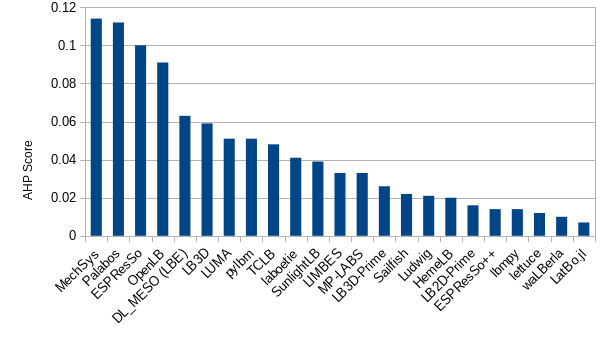
\includegraphics[width=1.0\textwidth]{installability_chart}
		\caption{AHP Installability Score}
		\label{Fig_Installability}
	\end{center}
\end{figure}

Figure \ref{Fig_Installability} shows the installability ranking of the software packages using AHP. Software packages with a higher score tend to have one set of linear installation instructions that is written as if the person doing the installation has none of the dependencies installed. The instructions often have compatible operating system versions listed and include instructions for the installation of dependencies. The top ranked packages also often incorporate some sort of the automation in the installation process and have fewer manual installation steps. The number of dependencies a package has does not correlate with a higher score. Installation validation, often through test examples with expected output, is correlated with a higher score.

Many software packages would benefit from a rewrite or reorganization of installation instructions. A single location for installation instructions would improve their maintainability and correctness. Listing compatible operating system and dependency versions would decrease installation time and errors, as would adding instructions on installing dependencies. Errors that may be encountered during the installation process need to prompt detailed messages or logs. Once a software package is installed, either a transparent automatic validation needs to be performed or the user needs to be able to perform a manual validation using test examples and output. Finally, uninstallation instructions should be included in the documentation. 
 
\subsection{Surface Correctness and Verifiability}

Sixteen of the software packages have a requirement specification or explicitly reference domain theory. This information is often found in a user manual, on a web page, or is mentioned in publications by the developers. In the latter case the user may need to spend significant time to find this information. 

Interviews with developers confirmed that many of the software packages were developed by domain experts with backgrounds in physics, mathematics and mechanical engineering. Many did not have formal software engineering education. Some development teams include computer scientists. Despite a lack of visible domain documentation and a resulting lower surface correctness and verifiability score, many software packages do have a strong domain background. 

Document generation tools are explicitly used by 12 software packages. Sphinx is used by 8 of them, and Doxygen is used by 7. Some of the packages use both.

Tutorials are available for all but 5 of the software packages. Generally they are linearly written and easy to follow. However, only 8 tutorials provided an expected output and it is not possible to verify the correctness of the output of the software packages that are missing this key information. In this case the user cannot be sure of correctness and may need to assume it if there are no immediately visible errors. 

Unit tests are only explicitly available for one of the software packages. Code modularization of most packages allows for a user to create tests with varying degrees of effort. These tests allow developers and users to verify the correctness of fragments of the source code, and in doing so better assess the correctness of the entire package.

The documentation or presence of continuous integration tools and techniques alludes to a more refined development process where faults are isolated and better recognized. On the surface only 2 of the packages mentioned applying the practice of continuous integration in their development process. 

Interviews with the developers of software packages suggest a more frequent use of both unit testing and continuous integration in the development processes than initially surveyed. For example, OpenLB, pyLBM, and TCLB use such methods during development despite it not being explicitly clear from a surface analysis. 

\begin{figure}[h!]
	\begin{center}
		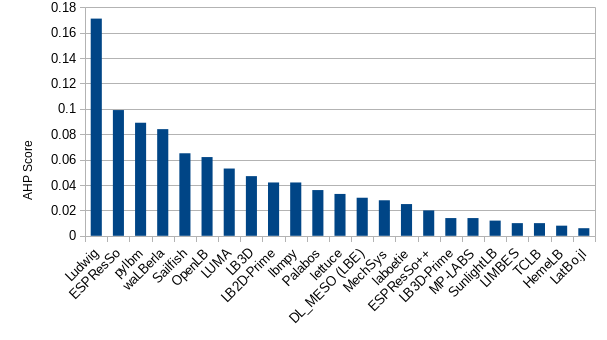
\includegraphics[width=1.0\textwidth]{correctnessverifiability_chart}
		\caption{AHP Surface Correctness and Verifiability Score}
		\label{Fig_CorrectnessVerifiability}
	\end{center}
\end{figure}

Figure \ref{Fig_CorrectnessVerifiability} shows the surface correctness and verifiability ranking of the software packages using AHP. Software packages with a higher score tend to have a visible requirements specification or references to theory documentation. They also explicitly use at least one document generation tool that builds confidence of correctness. The top ranked software packages all include an easy to follow getting started tutorial in their documentation, and most provide expected output for these tutorials. Only the top ranked package, Ludwig, provided unit testing. It and the second ranked package, ESPResSo, explicitly incorporated continuous integration in the development process. During developer interviews it was discovered that some other packages also use continuous integration and unit testing, despite not being explicitly stated in documentation. Such packages, including OpenLB, pyLBM, and TCLB, have higher true correctness and verificablity than is noted from surface analysis.

The inclusion of requirements specification and theory documentation greatly benefits the correctness and verifiability of software packages. The use of document generation tools can help build confidence in correctness. The addition of easy to follow tutorials, along with expected output, further helps users verify the software and have confidence in its correctness. Unit testing documentation and capability, as well as the use of continuous integration tools and techniques such as Bamboo, Jenkins, and Travis CI, help verify correctness. Several interviewed developers alluded to difficulty with testing large numbers of features, and some even manually tested output. The use of well defined unit testing tools could decrease the time spent testing some feature.

\subsection{Surface Reliability}

Errors occurred when installing 16 of the software packages, and every instance prompted a message. Error messages included unrecognized commands (even when following the installation guide), missing links, missing dependencies, syntax errors in code files, and vague output. Several automatic installation processes could not find and load dependency packages. The installation files pointed to outdated external repositories. Seven of the installations were clearly recovered and one of the installations was assumed to be recovered due to the absence of installation verification. The installation of eight of the software packages could not be recovered. Most of these installations could not reach a dependency repository, had an incompatible error in their core installation files, or prompted vague error messages. 

Of the 13 software packages that installed correctly and had tutorials, 4 broke during tutorial testing. All four error resulted in an error message being displayed. One error was due to a missing tutorial dependency, another was due to an invalid command despite following the tutorial, and the final two errors were execution errors. Of the 4 broken tutorial instances, only the one that was missing a dependency was recoverable. 

\begin{figure}[h!]
	\begin{center}
		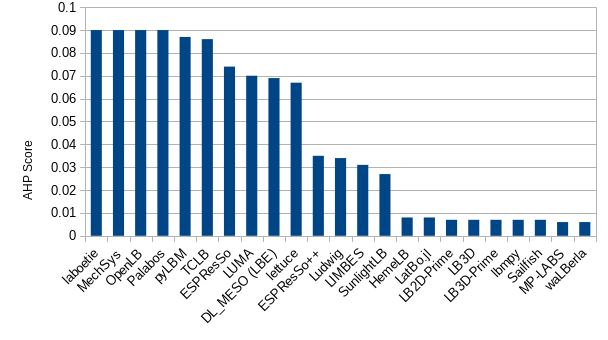
\includegraphics[width=1.0\textwidth]{reliability_chart}
		\caption{AHP Surface Reliability Score}
		\label{Fig_Reliability}
	\end{center}
\end{figure}

Figure \ref{Fig_Reliability} shows the surface reliability ranking of the software packages using AHP. Software packages with a high score did not break during installation, or the installation was recoverable. All of the top 5 ranked packages had tutorials. One of these packages, pyLBM, broke during tutorial testing, but a descriptive error message helped in recovery.

Overall, lower ranked software packages were lacking clear documentation, testing or tutorial examples, and descriptive error messages, and had broken automatic dependencies. Thus, regarding surface reliability, software packages would benefit from clear up-to-date installation and tutorial documentation, and descriptive error messages.

\subsection{Surface Robustness}

The software packages were tested to handle unexpected input, including incorrect data types, empty input, and missing files or links. Success predicated on a reasonable response from the system, including appropriate error messages and an absence of unrecoverable system failures. 

\begin{figure}[h!]
	\begin{center}
		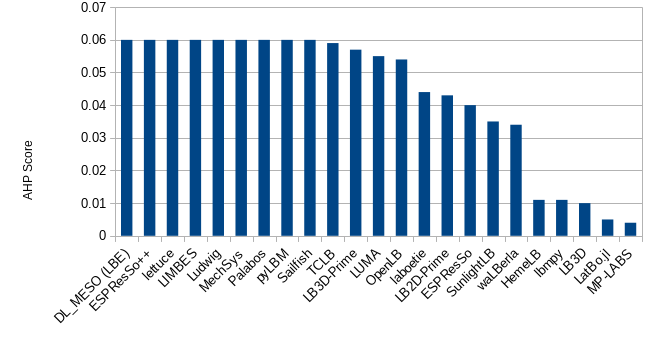
\includegraphics[width=1.0\textwidth]{robustness_chart}
		\caption{AHP Surface Robustness Score}
		\label{Fig_Robustness}
	\end{center}
\end{figure}

Figure \ref{Fig_Robustness} shows the surface robustness ranking of the software packages using AHP. Software packages with a high score behaved reasonably in response to unexpected input as described above. All of the software packages that installed correctly passed this test. They output descriptive error messages or did not crash. Software packages with a lower surface robustness score had not installed correctly, so their score here may not be a true reflection of runtime robustness. Similarly, all software packages that installed correctly and require plain text input files handled an unexpected change, a replacement of new lines with carriage returns, to these input files correctly. 

\subsection{Surface Performance}

Each software package was not quantitatively measured for surface performance.
Although the software packages all apply Lattice Boltzmann methods to solve scientific computing problems, the packages focus on varied domains, with varying parameters, and are technically different from each other. Due to this, a comparison of performance is not appropriate. Instead, in this project we looked through each software package's artifacts for evidence that performance was considered. The artifacts of 17 software packages mentioned the use of some sort of parallelization for execution. This included GPU processing and the CUDA parallel computing platform. GPUs provide superior processing power and speed compared to CPUs, and are often used for scientific computing when a large amount of data is involved. The software package TCLB is implemented in a highly efficient multi-GPU code to achieve performance suitable for model optimization \citep{rutkowski2020open}. In the Ludwig package, a so-called mixed mode approach is used where fine-grained parallelism is implemented on the GPU, and MPI is used for even larger scale parallelism \citep{gray2013ludwig}. While some software packages required CUDA and GPU processing, some had the option of using either the GPU or the CPU. The packages that require GPU and CUDA have better performance at the expense of installability and surface reliability.

\subsection{Surface Usability}

Software package artifacts were reviewed for the presence of a tutorial, a user manual, documented user characteristics, and a user support model. In total 18 software packages have a tutorial and 13 have a user manual. The tutorials vary in scope and substance, and 8 include an expected output to compare user results to. Most user manuals are in the form of a file that can be downloaded, while some are rendered on a web-page. Some packages do not have a user manual but do have useful documentation distributed on their web-pages. Expected user characteristics are documented in 4 software packages. Users are typically scientists or engineers trying to test a new application. Their background is often physics, chemistry, biophysics, or mathematics. All but one of the packages have a user support model, and several of them have multiple avenues of user support. The most popular avenue of support is git, followed by email and forums. One software package has a FAQ page.    

\begin{figure}[h!]
	\begin{center}
		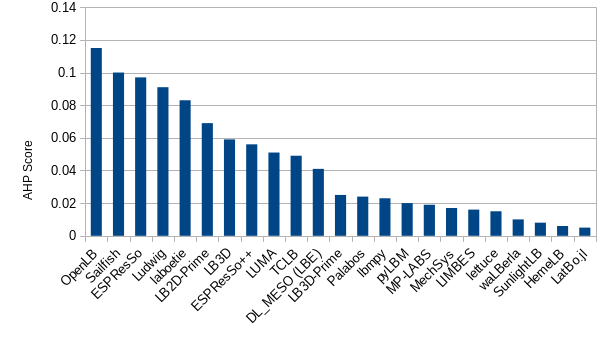
\includegraphics[width=1.0\textwidth]{usability_chart}
		\caption{AHP Surface Usability Score}
		\label{Fig_Usability}
	\end{center}
\end{figure}

Figure \ref{Fig_Usability} shows the surface usability ranking of the software packages using AHP. Software packages with a high score have a tutorial and user manual, and sometimes have documented user characteristics, and have at least one user support model, with many having several. 

Interviews with developers revealed several usability issues. Some users have misunderstood boundaries of LBM and computational fluid dynamics in general, and have combined or applied methods that are not physically sound together. Sometimes users have applied LBM to poorly defined or inappropriate fluid dynamics problems. The users do not realize the limitations of the methods, of the software, and of how much time and effort is required to properly model a problem that can technically be modeled by the software. The software is not as easy as out of the box plug and play. Developers of some of the software packages mitigated this by editing the source code to prevent unsound combination from being applied, and by updating the documentation to better inform users of LBM limitations, and of the requirements to properly model appropriate problems, including what algorithms and parameters to use. 

Some additional infrequent software usability issues were commented on. Users have had trouble with installation and understanding how to maneuver the interfaces and how to set up or run models. These issues are addressed by various user support models, including frequently asked questions sections on the software package websites, user guides, and hardware and software requirement specifications.

One software package changed its scripting language to Python to make it more usable. The developer commented that this was the biggest step in addressing usability, commenting that Python was a much easier language for users to learn and understand. 

\subsection{Maintainability}

Software packages were reviewed for the presence of artifacts. Every type of artifact or file that is not a code file was recorded. The software packages were also reviewed for version numbers. This information could be used to better troubleshoot software issues and organize documentation. All but 3 software packages have source code release and documentation version numbers. 

Information on how code is reviewed, or how to contribute to the project was also noted. In total, eleven software packages have this information, which was found in various artifacts, including in developer guides, contributor guides, user guides, developer web-pages, and README files. 

Issue tracking is used in 22 software packages, 15 of which use git, 6 use email, and one uses SourceForge. Most software packages that use git have most of their issues closed, and only 3 have less than 50 percent of their issues closed. Furthermore, most packages that use git for issue tracking use GitHub as a version control system, one package uses CVS for issue tracking, and 8 packages do not appear to use any such system.

Software package code files were further measured for the percentage of code that is comments. Packages with a higher percentage of comments were designated as more maintainable. Comments represent more than 10 percent of code files in 15 packages, and the average percentage of comments is 13.7.


\begin{figure}[h!]
	\begin{center}
		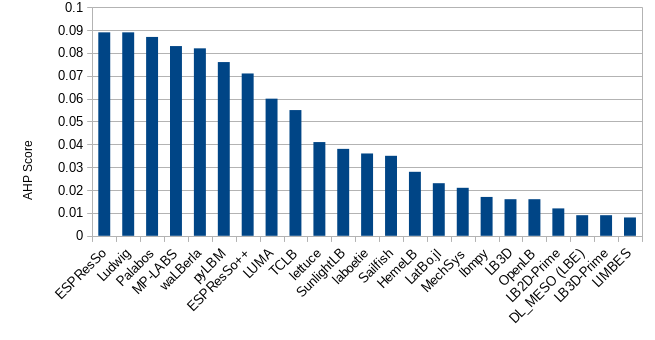
\includegraphics[width=1.0\textwidth]{maintainability_chart}
		\caption{AHP Maintainability Score}
		\label{Fig_Maintainability}
	\end{center}
\end{figure}

Figure \ref{Fig_Maintainability} shows the maintainability ranking of the software packages using AHP. Software packages with a high score provide version numbers on documents and source code releases, have an abundance of high quality artifacts, and use an issue tracking tool and version control system. These packages also appear to reasonably handle tracked issues, having most of their issues closed. Their code files are well commented with more than 10 percent of the code being comments. 

Interviews with developers revealed that most projects do have a defined process for accepting contributions from current team members or those that at some time had been linked to the packages or developers. The packages rarely get contributions from outside developers, but the process would be similar as for the aforementioned group.

Contributions are made through GitHub, and are then reviewed and pulled by lead developers, often with consultation with a group of core developers depending on the organizational model. Continuous integration is part of the process for some packages. 

Some developers noted that their software package does not have well defined contributing guide in the repository but it might be a good idea to add one in the near future. They would be very happy to see spontaneous contribution from outside of their organization, but now it is currently not the case.

Furthermore, maintainability has been addressed by increasing source code modularity, reducing duplicate information, and improving abstraction. Several software packages have had large sections of their code base redeveloped with languages that the developers felt are more understandable and readable, and that are better supported and have preferred dependencies. Data structures have also been redeveloped and storage has been improved. One software developer mentioned that the mathematical foundations that the geometries and models are designed from have been re-evaluated and optimized. 

\subsection{Modifiability}

Software packages were not quantitatively measured for modifiability.
In this project we asked developers to comment on modifiability when we interviewed them. Specifically, we asked if ease of future changes to the system, modules, and code blocks was considered when designing the software. We also asked if any measures had been taken to ensure the ease of future changes. 
All of the developers that were interviewed noted that the ease of future changes was considered and that measures to ensure it had been taken.

A high degree of code modularity and abstraction was noted by one developer as a measure to ensure ease of future changes. They also noted that some of the code base was transitioned from c to c++, which could ease modifiability of that software package. Another developer noted that their software package was designed to easily allow for the addition of some LBM features, but changes to major aspects of the LBM models would be difficult. Furthermore, the package was designed with flexible data structures and storage in mind. 

Some software packages, like Palabos, provide validation benchmarks for their core fundamental algorithmic ingredients \citep{latt2021palabos}. The stated intent of these benchmarks is to showcase the validity and usefulness of the package in order to stimulate the development of third-user extensions. The Palabos package identifies as as a development framework for modeling problems in various computational fluid dynamics areas. 

\subsection{Reusability}

The total number of source code files was measured for each software package. A larger number of source files was associated with increased reusability since this generally represented either more software package functionality or better modularization. The software packages were also reviewed for the presence of API documentation, which indicates that a software package was developed with interaction between other software applications in mind. 

\begin{figure}[h!]
	\begin{center}
		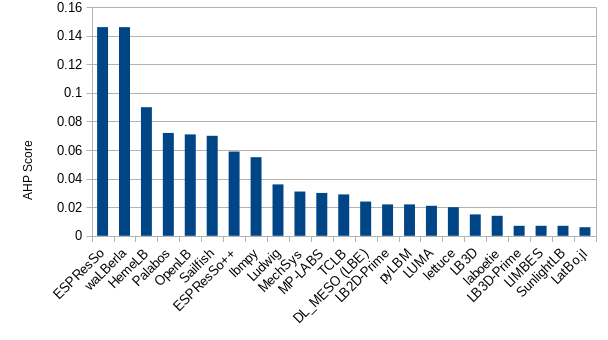
\includegraphics[width=1.0\textwidth]{reusability_chart}
		\caption{AHP Reusability Score}
		\label{Fig_Reusabilty}
	\end{center}
\end{figure}

Figure \ref{Fig_Reusabilty} shows the reusability ranking of the software packages using AHP. Software packages with a high score have thousands of source code files and API documentation. The highest scoring packages, ESPResSo and waLBerla, have extensive functionality, including graphical visualizations as well as modeling that does not use LBM. For this reason a comparison between other software packages is not on a level field, but regardless of this these packages do have an abundance of reusable components. 

There was a strong focus on modularity when designing the waLBerla framework in order to enhance productivity, reusability, and maintainability \citep{bauer2021walberla}. The software design has enabled for waLBerla to be successfully applied in several projects as a basis for various extensions \citep{bauer2021walberla}.

\subsection{Surface Understandability}

Ten random source code files of each software package were reviewed for several measures. This measure of surface understandability may not perfectly reflect each package due to this limitation. All of the packages appear to have a consistent indentation and formatting style. Only LUMA and HemeLB explicitly identify coding standards that are used during development. Generally, the software packages use consistent, distinctive, and meaningful code identifiers. Only 4 packages appear to use vague identifiers. Hard coded constants were observed in the source code of 12 packages. The constants are used for various parameters, mathematical constants, and matrix definitions. All of the packages are well commented. Comments clearly indicate what is being done. Domain algorithms are noted in the source code of 11 packages. All of the packages were well modularized. When observing the source code files, it was found that 13 of the packages had a consistent style and order for function parameters.

\begin{figure}[h!]
	\begin{center}
		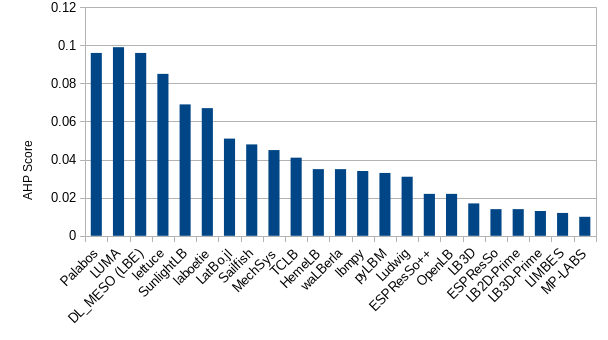
\includegraphics[width=1.0\textwidth]{understandability_chart}
		\caption{AHP Understandability Score}
		\label{Fig_Understandability}
	\end{center}
\end{figure}

Figure \ref{Fig_Understandability} shows the surface understandability ranking of the software packages using AHP. Software packages with a high score have a consistent indentation and formatting style, and consistent, distinctive and meaningful code identifiers. They also have hard coded constants, and explicitly identify mathematical and LBM algorithms. Their comments are clear and indicative of what is being done. The source code is well modularized and structured.  

Software developers noted that in their opinion users have generally found their packages to be understandable. One developer commented that some users have attempted to run physically incompatible LBM methods, and the solution was to edit the code to prevent such combinations, as well as update the documentation to prevent misunderstanding the methods. Similarly, another developer noted that some users had issues setting up parameters for LBM schemes. The solution was to this was to update the interface where these parameters are set, as well as adding functionality to test the stability of the parameters. A third developer noted that some users lack the background knowledge to easily model flow problems using their software. A frequently asked questions section was added to the source package website to help users find answers to common questions. The package also has detailed documentation, including guides and usage requirements specification.

\subsection{Traceability}

Software packages were not quantitatively measured for traceability.
In this project we asked developers to comment on traceability when we interviewed them. They were asked to comment on their documentation and how it fits into their development process. 

One developer noted that all major additions to their package had accompanying changes to artifacts, especially noting user documentation, and how it is updated to note major usability issues. Considerable effort had been put into the documentation. They want to lower the entry barrier for new developers so there is considerable documentation aimed at developers, and it is frequently updated. This documentation informs developers on how to get started, orients them to the artifacts, source code, and system architecture, as well as how the software package build system works, and how the coupling between the simulation engine and the interface works. 

Another developer noted the importance of documentation for both user and developers of their software. New features are always well documented in the artifacts. The developers use documentation to stay up to date on the status of the software package, and to expand or use features, like computational models or algorithms. This is necessary so that the coding standard for these models is kept consistent as developers come and go.

The importance of documentation for both users and developers was stressed throughout the interviews. However, it was noted several times that a lack of time and funding had negative affect on the documentation. Most of these developers are scientific researchers evaluated on the scientific papers that they produce. Writing and updating documentation is something that is done in free time, if that time arises, and if writing documentation is a concern. Sometimes it is a last priority for the developers. Finding ways to hasten updating documentation would increase the frequency of such updates and benefit both users and developers. 

One developer noted the use of documentation generators like Doxygen. It would be advisable for more projects to use such automatic document generation tools, if they are a good technological fit.  

\subsection{Visibility and Transparency}

Software package artifacts were reviewed for the identification of a specific development model, like a waterfall of agile development model, and the presence of documentation recording the development process and standard. They were also reviewed for the identification of the development environment, and the presence of release notes. The packages tended to not explicitly use well-known development models. This was also noted in the interviews with developers detailed below. The development teams of these packages are fairly small and easily organized without the need for such processes. Seven of the software packages did have some artifacts outlining the general development process, how to contribute, and the status of the package or its components. Eight of the packages have artifacts that note the development environment. While this information could help developers, and would improve transparency, the small close-knit nature of the development teams make explicitly publicly specifying this information practically unnecessary. Version release notes were found in 9 of the software packages.

\begin{figure}[h!]
	\begin{center}
		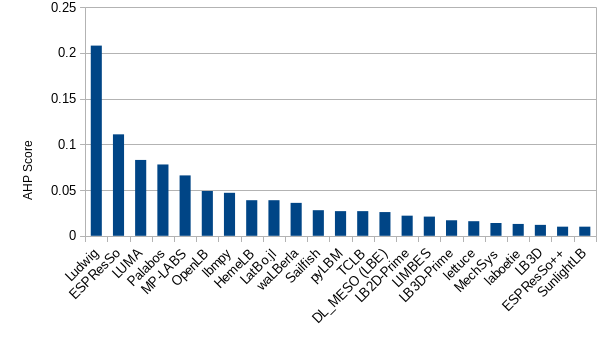
\includegraphics[width=1.0\textwidth]{visibilitytransparency_chart}
		\caption{AHP Visibility and Transparency Score}
		\label{Fig_VisibilityTransparency}
	\end{center}
\end{figure}

Figure \ref{Fig_VisibilityTransparency} shows the visibility and transparency ranking of the software packages using AHP. Software packages with a high score have an explicit development model and defined development process. They also 
had detailed and easy to access notes accompanying software releases. 

Developers were asked to comment on the obstacles in their development process. One developer noted that a lot of their source code had been written with a specific application in mind, and that there is too much coupling between components. Addressing this issue would help with code modifiability and reusability. Updating the development process would help resolve this issues and prevent such issues in the future. Improving the visibility of software changes and the peer review process would also help. Improving the software engineering education or experience of developers is also an idea that was brought up by several developers. Specifically, developers should always write code that is decoupled and modular, and should keep in mind the visibility of their contributions by better updating documentation and ensuring that their contributions are transparent to the rest of the developers. This would help catch issues in the code contributions, and improve source code maintenance.   

According to one developer, some obstacles to the development processes of their package had been overcome by the introduction of continuous integration practices, and a peer review process for contributions. These practices decrease development and maintenance times. Another developer mentioned that their package had two sets of code, for executing the models on the CPU and GPU, and that maintenance was decreased by introducing macros, the use of which is now part of the development process. 

Developers were also asked how documentation fits into their development process. Several developers noted that developer documentation plays an important role in familiarizing potential contributors to the software system architecture. Without the guidance that the documentation provides it would be unlikely that contributions would pass the peer review process. 

None of the software packages whose developers were interviewed have a formal software development model. The packages all have fairly small development teams. These teams do accept outside contributors, but generally the teams are tight-knit, often working at the same institution, although one of the packages has an international team. One developer noted that while no formal model is used, their development model is something similar to a combination of agile and waterfall development models. 

The developers noted similar project management processes. In teams of only a couple of developers, the addition of new features or major changes were discussed with the entire team. Projects with more than a couple of developers had lead developer roles. These lead developers would review potential additions to the software. The software packages use GitHub for managing the project. Typically there are several development branches as well as the master branch.

\subsection{Reproducibility}

Software packages were not quantitatively measured for reproducibility.
In this project we asked developers to comment on reproducibility when we interviewed them.

Developers were asked if they have any concern that their computational results would not be reproducible in the future, and if they had taken any steps to ensure reproducibility.

One developer noted that they compare the results of their methods against manually calculated results. These tests comparing these results are automatically run for all source code changes that are suggested. The tests are run when a pull request is opened on GitHub. Even once these tests are complete, a peer review process is done before changes are fully committed to the appropriate branch. The results for all of the LBM schemes on the software package development branch are also compared daily for correctness, ensuring that the system output reflects the expected output.  

Several developers noted that they currently do not have a system in place to test for reproducibility, but it is of interest and could be implemented in the future. Generally, the mathematical foundations of the models are verified, but the output of the software packages is not compared to other output. Depending on the package and how it outputs LBM solutions, it may not be practical or feasible. A correct output may not be exactly reproducible, as it may be dependent on a probability distribution, so strictly comparing results may not be appropriate. 

The source code and artifacts of some software packages may be reproducible. There is considerable variance in the quality of the software specification and other developer documentation. Some packages are well detailed, and translating the specification into source code will produce similar results across developers. 

\subsection{Unambiguity}

Software packages were not quantitatively measured for unambiguity.
In this project we asked developers to comment on unambiguity when we interviewed them.

Developers were asked if they thought that the current documentation can clearly convey all necessary knowledge to the users, and if they had taken any steps to ensure clarity. 

One developer noted that their documentation was meant for users that are already familiar with underlying physics and computational fluid dynamics methods, and that these concepts are not explained in detail. The documentation focuses solely on how to technically use the software package, and includes a user guide and tutorial walk through of how to set up and run a simulation. With this in mind the developer believes that their documentation is in reasonable shape for a those with a minimum knowledge of the underlying physics to learn to use the package. If new users have technical questions these can be addressed in further revisions of the documentation. New developers should also find that the code documentation is reasonably clear and useful. Information that is missing, like information explaining dependency packages, is reasonably referenced. 

Another developer also noted that their documentation was in reasonable shape, but they would really appreciate more user feedback to improve it. They also noted that they believe a lack of knowledge of the underlying physics and computational fluid dynamics concepts can be an issue for some users. This information can be referenced in the documentation, but it is not something that the documentation needs to detail. 

\subsection{Overall Quality}

Figure \ref{Fig_OverallScore} shows the overall ranking of the software packages using AHP. Software packages with an overall high score had ranked high in at least several of the individual qualities that were quantitatively measured.

\begin{figure}[h!]
	\begin{center}
		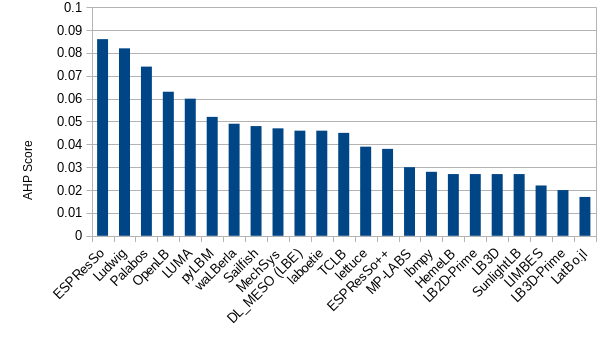
\includegraphics[width=1.0\textwidth]{finalscore_chart}
		\caption{AHP Overall Score}
		\label{Fig_OverallScore}
	\end{center}
\end{figure}

Looking at the top three ranked packages. ESPResSo had achieved a relative high score in installability, surface correctness and verifiability, surface usability, maintainability, reusability, and visibility and transparency. Ludwig scored high in surface correctness and verifiability, surface robustness, surface usability, maintainability, and visibility and transparency. Palabos scored high in installability, surface reliability, surface robustness, maintainability, and understandability. 

Section \ref{qualityrecommentations} further analyzes these findings and offers some software quality recommendations for future development of LBM software.

\newpage

\section{Answers To Research Questions}\label{answersquestions}

\subsection{Artifacts Present - DONE 1st DRAFT}\label{artifacts}

The software packages were examined for artifacts. Below we have grouped these into common, less common, and rare artifacts. Common artifacts were found in 16 to 23 of the software packages. Less common artifacts were found in 8 to 15 of the software packages. Rare artifacts were found in 1 to 27 of the software packages. 

\subsubsection{Common Artifacts}
The following artifacts were commonly found in the 23 software packages that were tested. All of the top four AHP ranked packages, ESPREsSo, Ludwig, Palabos, and OpenLB have each of these artifacts, except for a clear requirements specification or theory notes. Only three of the packages were found to have that artifact. 

\begin{singlespace}
\begin{multicols}{2}	
\begin{itemize}
	\item Authors/Developers List
	\item Bug Tracker
	\item Dependency Notes 
	\item Installation Guide/Instructions 
	\item License
	\item List of Related Articles/Publications 
	\item Makefile / Build File 
	\item README File 
	\item Requirements Specification / Theory Notes
	\item Tutorial
\end{itemize}
\end{multicols}
\end{singlespace}

These common artifacts contribute to the quality of the software in various ways. A list of authors and developers helps potential users and contributors more easily contact project members to answer questions affecting many software qualities. A bug tracker helps with organizing improvements to the software, also improving many software qualities. Dependency notes help users install the software, as does an installation guide. Makefiles or other automated build files decrease human error in the installation process. Visible licenses promote usage of the software. Requirements specifications, linked theory notes, and related articles and publications help clarify the software and make it more understandable, decrease ambiguity, and help to verify its correctness. README files also help with understandability. Meanwhile tutorials help users become familiar with using the software.


\subsubsection{Less Common Artifacts}
The following artifacts were less commonly found in the 23 software packages that were tested. The top four AHP ranked packages have most of these artifacts.
Only one of those four packages does not have a user manual or guide, but it does have a detailed and informative website. Another one of the top four packages does not have any visible design documentation. A third package from that list does not appear to use a version control system. It is probably that such a system is in use but is not visible outside of the development team since the package website notes a current version number. 

\begin{singlespace}
	\begin{multicols}{2}	
		\begin{itemize}
			\item Change Log / Release Notes
			\item Design Documentation
			\item Functional Specification/Notes	
			\item Performance Information/Notes
			\item Test Plan/Report/Script/Data/Cases
			\item User Manual/Guide
			\item Version Control
		\end{itemize}
	\end{multicols}
\end{singlespace}

These artifacts also contribute to software quality. A change log or release notes improve traceability of the software. Design documentation helps with maintaining, modifying, and reusing the software. Version control also helps to improve these qualities, as well as traceability. Functional specifications and notes clarify the software, contributing to usability and understandability. A user manual also benefits those qualities and with installability, and correctness and verificability. Performance notes suggest that performance was considered when developing the software. Test plans, scripts, and cases, help verify correctness. 


\subsubsection{Rare Artifacts}
The following artifacts were rarely found in the 23 software packages that were tested. It is not common for the top four AHP ranked packages to have many of these artifacts. None of the top four packages have any explicit API documentation. Three of these packages have information on contributing to the project. Two of them have a FAQ section or forums. One has verification and validation notes and a video guide explaining how to use the software. 

\begin{singlespace}
	\begin{multicols}{2}	
		\begin{itemize}
			\item API Documentation
			\item Developer/Contributing Manual/Guide
			\item FAQ / Forum
			\item Verification and Validation Plan/Notes
			\item Video Guide (including YouTube)
		\end{itemize}
	\end{multicols}
\end{singlespace}

Although these artifacts were rarely found in our set of LBM software, they also contribute to software quality. API documentation helps with reusing the software. Developer and contributor manuals and guides help with maintainability, visibility and transparency. FAQs and forums increase usability of software. Verification and validation notes can be used to help check if a system meets specifications. Video guides can contribute to many software qualities, depending on the content of the video. 

\subsection{Tools Used - DONE 1st Draft}
The purpose of tools is to support the development, verification, maintenance, and evolution of software, software processes, and artifacts \citep{ghezzi1991fundamentals}. Many tools are used by current LBM software packages. The tools noted here are subdivided into development tools, dependencies, and project management tools.

\subsubsection{Development Tools}

These tools support the development of end products but do not become part of them, unlike dependencies that remain in the application once it is released \citep{ghezzi1991fundamentals}. The following type of development tools were explicitly noted in the artifacts or web pages of the 23 LBM packages that were assessed. It is likely that other tools, such as debuggers, were used but are not specified here.

\begin{singlespace}
	\begin{multicols}{2}	
		\begin{itemize}
			\item Continuous Integration Tools
			\item Code Editors
			\item Development Environment
			\item Runtime Environments
			\item Compilers
			\item Unit Testing Tools
			\item Correctness Verification Tools
		\end{itemize}
	\end{multicols}
\end{singlespace}

The use of the above tools can verify the correctness of software during its development. Only two of the software packages that were assessed mentioned using continuous integration tools like Travis CI. Code editors and compilers were explicitly noted to have been used by several packages, and were likely used by all of them. One of the packages explicitly noted the use of unit testing, but did not specify the tool that was used. Likewise the use of a tool for verifying the correctness of output was noted by one of the developers. It is likely that similar tools were used when developing other members of the software package list. 

\subsubsection{Dependencies}

The following types of dependencies were explicitly noted in the artifacts or web pages of the 23 LBM packages that were assessed. It is possible that other types of dependencies are part of these software packages but are not clearly specified in their artifacts or web sites and because of that they are not listed here.

\begin{singlespace}
	\begin{multicols}{2}	
		\begin{itemize}
			\item Build Automation Tools
			\item Technical Libraries
			\item Domain Specific Libraries
		\end{itemize}
	\end{multicols}
\end{singlespace}

Most of the software packages use some sort of build automation tools, most commonly Make. They also all use various technical and domain specific libraries. Technical libraries include visualization, data analysis, and message passing libraries among others. Domain specific libraries are scientific computing libraries. Specific libraries are not listed here but they fall into the above categories. Libraries that are not explicitly stated in any artifact may fall outside of the categories. 

\subsubsection{Project Management Tools}

Many of the software packages that were assessed were developed by teams of two or more people. Their work needed to be coordinated and managed. The following types of project management tools were explicitly noted in the artifacts, web pages, or interviews with the developers of the 23 LBM packages that were assessed. As with development tools and dependencies, it is possible that other types of project management tools were used to coordinate and manage the projects but are not specified and because of that they are not listed here.

\begin{singlespace}
	\begin{multicols}{2}	
		\begin{itemize}
			\item Collaboration Tools
			\item Email
			\item Change Tracking Tools
			\item Version Control Tools
			\item Document Generation Tools
		\end{itemize}
	\end{multicols}
\end{singlespace}

Collaboration tools are noted to have been used when developing the software projects. Most often email and video conferencing is used. Project management software was not explicitly mentioned, but it is possible that some of the project use such software. Many of the projects are located on GitHub, and it's developers use the platform to help manage their projects, especially bug related issues. Most of the projects appear to use change tracking and version control tools. They often use GitHub for this, and a few use Git or CVS. Document generation tools are mentioned in the artifacts of 12 of the projects. Tools such as Sphinx and Doxygen are explicitly used in this capacity. Drasil could be considered as an alternative to generate artifacts since it is geared specifically towards research software domains like LBM software. 


\subsection{Principles, Processes, and Methodologies - DONE 1st DRAFT}

Most of the assessed software packages do not explicitly state in their artifacts the motivations or design principles that were considered when developing the software. One package, Sailfish, indicates that shortening development time was considered in early stages of design, with the developers opting for using Python and CUDA/OpenCL to achieve this without sacrificing any computational performance. The goals of that project are explicitly listed as performance, scalability, agility and extendability, maintenance, and ease of use. The project scored well in these listed categories during our assessment, for the categories that were measured. 

Processes, like methods, are ways of doing things, especially in an orderly way; while methodologies are defined as systems of methods \citep{ghezzi1991fundamentals}. It is not explicitly indicated in the artifacts of most of these packages that development involved following any specific model, like a waterfall of agile development model. One developer noted that while no formal model is used, their development model is something similar to a combination of agile and waterfall development models. The developers teams of the LBM packages are fairly small and easily organized without the need for such methodologies. 

Seven of the software packages contain artifacts outlining the general development process, like basic instructions on how to contribute. Most of the development teams accept outside contributors, but generally the teams are tight-knit, often working at the same institution. 

The developers that were interviewed all noted similar project management processes. In teams of only a couple of developers, the addition of new features or major changes are discussed with the entire team. Projects with more than a couple of developers have lead developer roles. These lead developers review potential additions to the software. One of the developers noted in their interview that a peer review process is used to review major changes and additions.

The software packages frequently use GitHub for managing the project. Typically there are several development branches and changes from these branches are merged into the master branch. 

Documentation was also noted as playing a significant role in the development process, specifically with on-boarding new developers. An intention is to lower the entry barrier for these new contributors. The documentation provides information on how to get started, orients the user to artifacts and the source code, and explains how the system works, including the so-called simulation engine and interface. The use of document generation tools is mentioned in the artifacts of 12 software packages, and was noted during interviews with developers. The mentioned document generation tools are Sphinx and Doxygen. 

Two types of software changes were noted during interviews. One is feature additions, which arise from a scientific or functional need. The development of these changes was noted to involve more formal discussions within the development team and the execution involves lead developers. The other change type is code refactoring, which only sometimes involves formal discussions with the development team. New developers were noted to play an increased role in these changes compared to the former changes. Software bugs are typically addressed in a similar fashion as code refactoring, and issue trackers are commonly used to manage these changes. 

Interviews with the developers of software packages also revealed a more frequent use of both unit testing and continuous integration in the development process than was found by only examining the artifacts. The use of automatic installation processes is also common. Most often this involved a Make script.


\subsection{Pain Points - DONE 1st Draft}

Developers were asked to comment on obstacles in their development process, obstacles encountered by user, and potential future obstacles with the software packages. 

Several development process obstacles were noted. One developer noted that their small development team, common in LBM software packages, has a lack of time to implement new features.  Team members are almost always part of the same institute or already know each other from other projects. External contributions are rare despite many of the projects accepting them.

A lack of software development experience was noted by the developer of a third package where many of the team members on the project are domain experts. There is a steep learning curve to get these team members to contribute good quality source code. This has been somewhat addressed as the code is now generally written in a way that the developer thinks makes it as easy as possible for contributions. 

The developer also noted that there is a lack of incentive and funding in academia for developing good scientific software that people end up using. There are no journals that publish such source code. There is no place for the development of good quality software. Scientific software is often developed by the researchers that temporarily use it in their own research and keep the development and use in-house. This software often does not meet the standards that would be required by external users. Sometimes the software is commercialized but it is not open source. 

Documentation is important, but it's quality could be improved. There is often no time or funding for maintaining quality documentation for software that is rarely used externally. Furthermore, documentation generally does not teach the underlying metaphysics. It sometimes provides an introduction to these topics. Users would need to already be familiar with these topics or spend time referencing suitable textbooks. The documentation generally focuses on explaining how to use the software. It is not feasible for package documentation to address the underlying metaphysics topics in detail. Sometimes frequently asked questions on the underlying theory are answered in the documentation, or pointers to answers are noted.

Technically, setting up parallelization was also noted as a pain point for one of the developers, and the introduction of continuous integration by another. Software development knowledge could mitigate some pain points. As already noted, many of the developers are domain experts and not professional software developers. An interviewed developer with more extensive software development experience noted that eliminating equivalent statements using macros had helped improve the quality of their source code, specifically helping with extending code to run on both the CPU and GPU. 

Difficulties with ensuring correctness were also noted by several developers. They indicated that tests are run on new additions,on  both the individual modules and on the entire system to verify continued system correctness. These tests compare the package output to known correct output using test cases. A developer commented that the amount of testing data that is needed for some cases is a problem, as free services do not offer capabilities to store and frequently process such large amounts of data and in-house testing solutions needed to be created.

A few obstacles related to users were found. Several developers noted that users sometimes try to combine LBM methods with cases incorrectly, and that this is not theoretically sound. Some users think that the packages will work out of the box to solve their cases, while the packages require a good understanding of computational fluid dynamics and significant effort in setting up each case. These packages are not like more commercial software packages, they are generally set up to solve specific research problems. While they are modifiable to solve similar problems, these modifications are not trivial. So far this has been addressed by updating the documentation to better inform users of the underlying LBM theory and package requirements. Similar issues with LBM parameters were noted by another developer. Updating the user interface to better explain explain theoretical principles, as well as test user input, was the implemented solution. As noted above, sometimes frequently asked questions on the underlying theory and on how to use the software are answered in the documentation.

One developer commented that parts of their source code had been refactored to Python partially to address usability. Python was perceived as a much more usable language that would be easy for future users and developers to learn and understand. According to this developer this was one of the biggest steps in terms of addressing usability.

A few potential future obstacles were noted. One developer said that their source code had been written with a specific application in mind and that there was too much coupling between components. This would have an impact on future modifiability and reusability when trying to extend the software. The effected code would need to be refactored.

As noted above, difficulties with ensuring future correctness could also arise. As new methods and functionality is added into the software, new test cases and test data will need to be developed and provided.


\subsection{Quality Recommendations - DONE 1st Draft}\label{qualityrecommentations}

The following points should be considered to improve LBM software quality.

\subsubsection{Installability}

\begin{itemize}
	\item Include OS compatibility, including versions.
	\item Include complete installation instructions.
	\item Include all dependencies in the installation instructions, required versions, and how to install them.
	\item If possible, automate the installation of dependencies.
	\item Installation instructions should be written as if the user does not have any dependencies installed and is installing on a clean OS.
	\item Limit installation instruction location to one location.
	\item Automate the installation process as much as possible.
	\item Include descriptive error messages for errors encountered during installation.
	\item Include a way to validate the installation.
	\item Include instructions for uninstalling the software.
\end{itemize}

\subsubsection{Surface Correctness and Verifiability}

\begin{itemize}
	\item Use a requirements specification document.
	\item Make public the requirements specification document, or explicitly reference the domain theory that the software is designed from.
	\item Ensure the above information is easy to find. Consider adding it to the user manual. 
	\item Development teams should include both domain experts and experiences software developers.
	\item Use and make public detailed documentation. Consider using automatic document generation tools.
	\item Include detailed tutorials with expected output.
	\item Use unit testing during development. Make public the facilities for unit testing.
	\item Modularize the source code.
	\item Use continuous integration tools and processes during development.
\end{itemize}

\subsubsection{Surface Reliability}

\begin{itemize}
	\item Include descriptive error messages where appropriate.
	\item In case automatic installation of dependencies fails, the system should indicate to the user what dependencies are needed and the installation procedure should be able to skip installing the dependencies after they have been manually installed.
	\item The packages should include detailed tutorials, including dependencies, expected output, and supplementary documentation.
\end{itemize}

\subsubsection{Surface Robustness}

\begin{itemize}
	\item Include descriptive error messages for cases of unexpected input  including incorrect data types, empty input, and missing files or links.
\end{itemize}

\subsubsection{Surface Performance}

\begin{itemize}
	\item Implement using parallelization tools. Consider GPU processing, CUDA, and MPI. 
	\item The user should be able to process the models on either the CPU or GPU.
\end{itemize}

\subsubsection{Surface Usability}

\begin{itemize}
	\item Include user hardware and software requirements.
	\item Include a user tutorial with expected output.
	\item Include a detailed user manual. Identify elements of user interfaces.
	\item Explicitly state the boundaries of the software, and intended applications.
	\item Identify appropriate fluid dynamics problems that can be solved by the software.
	\item Provide background domain information or a reference to it.
	\item Explicitly state the requirements and commitments required of the user to properly model their problem.
	\item Document expected user characteristics.
	\item Keep documentation in one location.
	\item Maintain a user support model (Git, email, forum, FAQ)
	\item If possible, consider using user-friendly scripting languages like Python. Especially in parts of the software that are likely to be modified or reviewed by users.
\end{itemize}

\subsubsection{Maintainability}

\begin{itemize}
	\item Include high quality artifacts. Ideally most of the common and less common artifacts listed in Section \ref{artifacts}.
	\item Include version numbers and release notes for all major releases. 
	\item Have a defined process for accepting contributions.
	\item Include documentation for making contributions to the project. 
	\item Use an issue tracker (Git, email, SourceForge, other) to manage bugs and changes. Issues should be closed regularly. 
	\item Use a version control system (GitHib, CVS).
	\item Source code needs to be well commented.
	\item Ensure source code is modular.
	\item Eliminate code duplication.
	\item If possible, develop using languages that are easy to read and quick to learn.
\end{itemize}

\subsubsection{Modifiability}

\begin{itemize}
	\item Ensure a high degree of code modularity and abstraction.
	\item If possible, develop using languages that are easy to read and quick to learn.
	\item Consider future modifiabilility in the design stage prior to any development.
	\item Consider flexibility of data structures and data storage in the design stage.
	\item Make public validation benchmarks.
\end{itemize}

\subsubsection{Reusability}

\begin{itemize}
	\item Modularize the source code.
	\item Document module interfaces.
	\item Provide API documentation, if applicable.
\end{itemize}

\subsubsection{Surface Understandability}

\begin{itemize}
	\item Maintain consistent formatting style across source code files.
	\item Identify a coding standard, if one is used during development.
	\item Use consistent, distinctive, and meaningful code identifiers. Identify algorithms that are used.
	\item Hard code domain constants.
	\item Add meaningful comments. They should indicate what is being done in each section of source code.
	\item Modularize the source code.
	\item Include user guides and usage requirements.
	\item In the documentation identify the limits of the software. 
	\item Identify the cases that the software can be applied to.
	\item Note the requirements of the user in order to set up their case. Identify what parameters are needed. 
	\item Consider adding a FAQ section to the documentation. 
\end{itemize}

\subsubsection{Traceability}

\begin{itemize}
	\item Update all relevant documentation when a change to the software is made.
	\item Use automatic document generation tools to limit the time spent on updating documentation.
	\item Include documentation aimed at developers, like a developers guide.
	\item Provide documentation that orients users and developers to artifacts, the source code, and system architecture.
	\item Highlight new system features between artifact versions. 
\end{itemize}

\subsubsection{Visibility and Transparency}

\begin{itemize}
	\item Identify the development model that was used, if one was used.
	\item Identify the development environment.
	\item Identify the development process and how to contribute. 
	\item Include notes with all releases.
	\item Write modular code.
	\item Communicate all contributions and changes to the entire development team.
	\item Use continuous integration processes and tools.
	\item Consider peer review processes for contributions. 
	\item Decrease code duplication.
	\item Maintain updated developer documentation.
	\item Make use of project management software.
\end{itemize}

\subsubsection{Reproducibility}

\begin{itemize}
	\item Compare results of methods against manually calculated or known correct results.
	\item Automate the above comparison. Run the comparison after code changes.
	\item Consider peer reviews for code contributions.
	\item Maintain detailed and up to date design documentation.
\end{itemize}

\subsubsection{Unambiguity}

\begin{itemize}
	\item Documentation must include all technical requirements and dependencies for using the software. 
	\item Documentation should detail how to properly use the software.
	\item Documentation should outline correct and incorrect use cases of the software.
	\item Documentation should either explain underlying CFD theories or reference appropriate resources.
	\item Consider asking users for feedback on the documentation.
\end{itemize}


\subsection{Designation Comparison}

answers last question of research questions:

How does software designated as high quality by this methodology compare	with top rated software by the community?


\newpage
\section{Conclusion}

- key findings restated
- comment on future work in state of the practice SCS

\newpage
\section{Appendix}
\begin{singlespace}
	
\subsection{Research Questions}\label{researchquestions}
	The following are the research questions that are considered. 
	
	\begin{enumerate}
		\item What artifacts are present in current software packages? 
		\item What tools (development, dependencies, project management) are used by current software packages?
		\item What principles, processes, and methodologies are used in the development
		of current software packages?
		\item What are the pain points for developers working on research software
		projects?  What aspects of the existing processes, methodologies and tools do
		they consider as potentially needing improvement?  How should processes,
		methodologies and tools be changed to improve software development and
		software quality?
		\item For research software developers, what specific actions are taken to
		address the following:
		\begin{enumerate}
			\item installability
			\item correctness and verifiability
			\item reliability
			\item robustness
			\item performance
			\item usability
			\item maintainability
			\item modifiability
			\item reusability
			\item understandability
			\item traceability
			\item visibility and transparency
			\item reproducibility
			\item unambiguity
		\end{enumerate} 
		\item How does software designated as high quality by this methodology compare	with top rated software by the community?
	\end{enumerate}

\newpage

\subsection{Measurement Template}\label{measurementtemplate2}
The table below lists the set of measures that are used to assess each software product. The first set identifies summary information, followed by 9 sets for software qualities and 3 sets for raw metrics. Each measure is followed by the type for a valid result. A superscript ∗ indicate that a response of this type needs to be accompanied by explanatory text. 

\captionof{table}{Measurement Template}\label{measurementtemplate}
\def\arraystretch{1.22}
\begin{tabular}{p{16cm}}
		\hline
		\textbf{Summary Information}\\
		\hline
		Software name? (string)\\
		URL? (URL)\\
		Affiliation (institution(s)) (string or {N/A})\\
		Software purpose (string)\\
		Number of developers (all developers that have contributed at least one commit to the project) (use repo commit logs) (number)\\
		How is the project funded? (unfunded, unclear, funded*) where * requires a string to say the source of funding\\
		Initial release date? (date)\\
		Last commit date? (date)\\
		Status? (alive is defined as presence of commits in the last 18 months) ({alive, dead, unclear})\\
		License? ({GNU GPL, BSD, MIT, terms of use, trial, none, unclear, other*}) * given via a string \\
		Platforms? (set of {Windows, Linux, OS X, Android, other*}) * given via string\\
		Software Category? The concept category includes software that does not have an officially released version. Public software has a released version in the public domain. Private software has a released version available to authorized users only. ({concept, public, private})\\
		Development model? ({open source, freeware, commercial, unclear})\\
		Publications about the software? Refers to publications that have used or mentioned the software. (number or {unknown})\\
		Source code URL? ({set of url, n/a, unclear})\\
		Programming language(s)? (set of {FORTRAN, Matlab, C, C++, Java, R, Ruby, Python, Cython, BASIC, Pascal, IDL, unclear, other*}) * given via string \\
		Is there evidence that performance was considered? Performance refers to either speed, storage, or throughput. ({yes∗, no})\\
		Additional comments? (can cover any metrics you feel are missing, or any other thoughts you have) \\
		\hline
\end{tabular}

\def\arraystretch{1.5}
\begin{tabular}{p{16cm}}
		\hline		
		\textbf{Installability  (Measured via installation on a virtual machine.) }\\
		\hline
		Are there installation instructions? ({yes, no})\\
		Are the installation instructions in one place? Place referring to a single document or web page. ({yes, no, n/a})\\
		Are the installation instructions linear? Linear meaning progressing  in a single series of steps. ({yes, no, n/a})\\
		Are the instructions written as if the person doing the installation has none of the dependent packages installed? ({yes, no, unclear})\\
		Are compatible operating system versions listed? ({yes, no})\\
		Is there something in place to automate the installation (makefile, script, installer, etc)? ({yes*, no})\\
		If the software installation broke, was a descriptive error message displayed? ({yes, no, n/a})\\
		Is there a specified way to validate the installation? ({yes*, no})\\
		How many steps were involved in the installation? (Includes manual steps like unzipping files) Specify OS. (number, OS)\\
		What OS was used for the installation? ({Windows, Linux, OS X, Android, other* }) *given via string\\
		How many extra software packages need to be installed before or during installation? (number)\\
		Are required package versions listed? ({yes, no, n/a})\\
		Are there instructions for the installation of required packages / dependencies? ({yes, no, n/a})\\
		Run uninstall, if available. Were any obvious problems caused? ({yes∗ , no, unavail})\\
		Overall impression? ({1 .. 10})\\
		Additional comments? (can cover any metrics you feel are missing, or any other thoughts you have)\\
		\hline
\end{tabular}

\def\arraystretch{1.33}
\begin{tabular}{p{16cm}}
	\hline		
	\textbf{Correctness and Verifiability}\\
	\hline
	Any reference to the requirements specifications of the program or theory manuals? ({yes∗ , no, unclear})\\
	What tools or techniques are used to build confidence of correctness? ({literate programming, automated testing, symbolic execution, model checking, assertions used in the code, Sphinx, Doxygen, Javadoc, confluence, unclear, other*}) * given via string\\
	If there is a getting started tutorial? ({yes, no})\\
	Are the tutorial instructions linear? ({yes, no, n/a})\\
	Does the getting started tutorial provide an expected output? ({yes, no*, n/a})\\
	Does your tutorial output match the expected output? ({yes, no, n/a})\\
	Are unit tests available?  ({yes, no, unclear})\\
	Is there evidence of continuous integration? (for example mentioned in documentation, Jenkins, Travis CI, Bamboo, other) ({yes*, no, unclear})\\
	Overall impression? ({1 .. 10})\\
	Additional comments? (can cover any metrics you feel are missing, or any other thoughts you have) \\
	\hline	
	\textbf{Surface Reliability}\\
	\hline
	Did the software “break” during installation? ({yes∗ , no})\\
	If the software installation broke, was the installation instance recoverable? ({yes, no, n/a})\\
	Did the software “break” during the initial tutorial testing? ({yes∗, no, n/a})\\
	If the tutorial testing broke, was a descriptive error message displayed? ({yes, no, n/a})\\
	If the tutorial testing broke, was the tutorial testing instance recoverable? ({yes, no, n/a})\\
	Overall impression? ({1 .. 10})\\
	Additional comments? (can cover any metrics you feel are missing, or any other thoughts you have)\\
	\hline		
	\textbf{Surface Robustness}\\
	\hline
	Does the software handle unexpected/unanticipated input (like data of the wrong type, empty input, missing files or links) reasonably? (a reasonable response can include an appropriate error message.) ({yes, no∗ })\\
	For any plain text input files, if all new lines are replaced with new lines and carriage returns, will the software handle this gracefully? ({yes, no∗, n/a})\\
	Overall impression? ({1 .. 10})\\
	Additional comments? (can cover any metrics you feel are missing, or any other thoughts you have)\\
	\hline
\end{tabular}

\def\arraystretch{1.4}
\begin{tabular}{p{16cm}}
	\hline		
	\textbf{Surface Usability}\\
	\hline
	Is there a getting started tutorial? ({yes, no})\\
	Is there a user manual? ({yes, no})\\
	Are expected user characteristics documented? ({yes, no})\\
	What is the user support model? FAQ? User forum? E-mail address to direct questions? Etc. (string)\\
	Overall impression? ({1 .. 10})\\
	Additional comments? (can cover any metrics you feel are missing, or any other thoughts you have)\\
	\hline	
	\textbf{Maintainability}\\
	\hline
	What is the current version number? (number)\\
	Is there any information on how code is reviewed, or how to contribute? ({yes*, no})\\
	Are artifacts available? (List every type of file that is not a code file – for examples please look at the ‘Artifact Name’ column of https://gitlab.cas.mcmaster.ca/SEforSC/se4sc/-/blob/git-svn/GradStudents/Olu/ResearchProposal/Artifacts\_MiningV3.xlsx) ({yes*, no, unclear}) *list via string\\
	What issue tracking tool is employed? (set of {Trac, JIRA, Redmine, e-mail, discussion board, sourceforge, google code, git, BitBucket, none, unclear, other*}) * given via string\\
	What is the percentage of identified issues that are closed? (percentage)\\
	What percentage of code is comments? (percentage)\\
	Which version control system is in use? ({svn, cvs, git, github, unclear, other*}) * given via string\\
	Overall impression? ({1 .. 10})\\
	Additional comments? (can cover any metrics you feel are missing, or any other thoughts you have)\\
	\hline		
	\textbf{Reusability}\\
	\hline
	How many code files are there? (number)\\
	Is API documented? ({yes, no, n/a})\\
	Overall impression? ({1 .. 10})\\
	Additional comments? (can cover any metrics you feel are missing, or any other thoughts you have)\\
	\hline
\end{tabular}

\def\arraystretch{1.4}
\begin{tabular}{p{16cm}}
	\hline		
	\textbf{Surface Understandability (Based on 10 random source files)}\\
	\hline
	Consistent indentation and formatting style? ({yes, no, n/a})\\
	Explicit identification of a coding standard? ({yes∗, no, n/a})\\
	Are the code identifiers consistent, distinctive, and meaningful? ({yes, no∗ , n/a})\\
	Are constants (other than 0 and 1) hard coded into the program? ({yes, no∗ , n/a})\\
	Comments are clear, indicate what is being done, not how? ({yes, no∗ , n/a})\\
	Is the name/URL of any algorithms used mentioned? ({yes, no∗ , n/a})\\
	Parameters are in the same order for all functions? ({yes, no∗ , n/a})\\
	Is code modularized? ({yes, no∗ , n/a})\\
	Overall impression? ({1 .. 10})\\
	Additional comments? (can cover any metrics you feel are missing, or any other thoughts you have)\\
	\hline		
	\textbf{Visibility/Transparency}\\
	\hline
	Is the development process defined? If yes, what process is used. ({yes∗, no, n/a})\\
	Are there any documents recording the development process and status?  ({yes∗, no}))\\
	Is the development environment documented? ({yes∗, no})\\
	Are there release notes? ({yes∗, no})\\
	Overall impression? ({1 .. 10})\\
	Additional comments? (can cover any metrics you feel are missing, or any other thoughts you have)\\
	\hline		
	\textbf{Raw Metrics (Measured via git\_stats)}\\
	\hline
	Number of text-based files. (number)\\
	Number of binary files. (number)\\
	Number of total lines in text-based files. (number)\\
	Number of total lines added to text-based files. (number)\\
	Number of total lines deleted from text-based files. (number)\\
	Number of total commits. (number)\\
	Numbers of commits by year in the last 5 years. (Count from as early as possible if the project is younger than 5 years.) (list of numbers)\\
	Numbers of commits by month in the last 12 months. (list of numbers)\\
	\hline
\end{tabular}

\def\arraystretch{1.4}
\begin{tabular}{p{16cm}}
	\hline		
	\textbf{Raw Metrics (Measured via scc)}\\
	\hline
	Number of text-based files. (number)\\
	Number of total lines in text-based files. (number)\\
	Number of code lines in text-based files. (number)\\
	Number of comment lines in text-based files. (number)\\
	Number of blank lines in text-based files. (number)\\
	\hline
	\textbf{Repo Metrics (Measured via GitHub)}\\
	\hline
	Number of stars. (number)\\
	Number of forks. (number)\\
	Number of people watching this repo. (number)\\
	Number of open pull requests. (number)\\
	Number of closed pull requests. (number)\\
	\hline
\end{tabular}

\newpage

\subsection{Grading Template}\label{gradingtemplate2}
The table below lists how each quality measure of the measurement template is used to calculate an overall impression in each software quality set.\newline

\captionof{table}{Grading Template}\label{gradingtemplate}
\def\arraystretch{1.5}
\begin{tabular}{p{16cm}}
	\hline		
	\textbf{Installability  (Measured via installation on a virtual machine.) }\\
	\hline
	Are there installation instructions? ({yes=1, no=-1})\\
	Are the installation instructions in one place? Place referring to a single document or web page. ({yes=1, no=0, n/a=0})\\
	Are the installation instructions linear? Linear meaning progressing  in a single series of steps. ({yes=1, no=0, n/a=0})\\
	Are the instructions written as if the person doing the installation has none of the dependent packages installed? ({yes=1, no=0, unclear=0})\\
	Are compatible operating system versions listed? ({yes=1, no=0})\\
	Is there something in place to automate the installation (makefile, script, installer, etc)? ({yes*=1, no=-1})\\
	If the software installation broke, was a descriptive error message displayed? ({yes=0, no=-2, n/a=1})\\
	Is there a specified way to validate the installation? ({yes*=1, no=0})\\
	How many steps were involved in the installation? (Includes manual steps like unzipping files) Specify OS. ($<$10 = 1)\\
	What OS was used for the installation? (does not count)\\
	How many extra software packages need to be installed before or during installation? ($<$10 = 1)\\
	Are required package versions listed? ({yes=1, no=0, n/a=1})\\
	Are there instructions for the installation of required packages / dependencies? ({yes=1, no=0, n/a=1})\\
	Run uninstall, if available. Were any obvious problems caused? ({yes∗=0, no=1, unavail=1})\\
	Overall impression? (a sum of $>$10 is rounded down to 10)\\
	\hline
\end{tabular}

\def\arraystretch{1.33}
\begin{tabular}{p{16cm}}
	\hline		
	\textbf{Correctness and Verifiability}\\
	\hline
	Any reference to the requirements specifications of the program or theory manuals? ({yes∗=2, no=0, unclear=0})\\
	What tools or techniques are used to build confidence of correctness? (any=1, unclear=0)\\
	If there is a getting started tutorial? ({yes=2, no=0})\\
	Are the tutorial instructions linear? ({yes=1, no=0, n/a=0})\\
	Does the getting started tutorial provide an expected output? ({yes=1, no*=0, n/a=0})\\
	Does your tutorial output match the expected output? ({yes=1, no=0, n/a=0})\\
	Are unit tests available?  ({yes=1, no=0, unclear=0})\\
	Is there evidence of continuous integration? (for example mentioned in documentation, Jenkins, Travis CI, Bamboo, other) ({yes*=1, no=0, unclear=0})\\
	\hline	
	\textbf{Surface Reliability}\\
	\hline
	Did the software “break” during installation? ({yes∗=0, no=5})\\
	If the software installation broke, was the installation instance recoverable? ({yes=5, no=0, n/a=0})\\
	Did the software “break” during the initial tutorial testing? ({yes∗=0, no=5, n/a=0})\\
	If the tutorial testing broke, was a descriptive error message displayed? ({yes=2, no=0, n/a=0})\\
	If the tutorial testing broke, was the tutorial testing instance recoverable? ({yes=3, no=0, n/a=0})\\
	\hline		
	\textbf{Surface Robustness}\\
	\hline
	Does the software handle unexpected/unanticipated input (like data of the wrong type, empty input, missing files or links) reasonably? (a reasonable response can include an appropriate error message.) ({yes=5, no∗=0})\\
	For any plain text input files, if all new lines are replaced with new lines and carriage returns, will the software handle this gracefully? ({yes=5, no∗=0, n/a=5})\\
	\hline		
	\textbf{Surface Usability}\\
	\hline
	Is there a getting started tutorial? ({yes=3, no=0})\\
	Is there a user manual? ({yes=4, no=0})\\
	Are expected user characteristics documented? ({yes=1, no=0})\\
	What is the user support model? FAQ? User forum? E-mail address to direct questions? Etc. (one=1, two+=2, none=0)\\
	\hline
\end{tabular}

\def\arraystretch{1.4}
\begin{tabular}{p{16cm}}
	\hline
	\textbf{Maintainability}\\
	\hline
	What is the current version number? (provided=1, nothing=0)\\
	Is there any information on how code is reviewed, or how to contribute? ({yes*=1, no=0})\\
	Are artifacts available? (List every type of file that is not a code file – for examples please look at the ‘Artifact Name’ column of https://gitlab.cas.mcmaster.ca/SEforSC/se4sc/-/blob/git-svn/GradStudents/Olu/ResearchProposal/Artifacts\_MiningV3.xlsx) (Rate 0 – 2 depending on how many and perceived quality)\\
	What issue tracking tool is employed? (nothing=0, email of other private=1, anything public or accessible by all devs (eg git) = 2)\\
	What is the percentage of identified issues that are closed? (50$\%$+=1, $<$50$\%$=0)\\
	What percentage of code is comments? (10$\%$+=1, $<$10$\%$=0)\\
	Which version control system is in use? (anything=2, nothing=0)\\
	\hline		
	\textbf{Reusability}\\
	\hline
	How many code files are there? (0-9=0, 10-49=1, 50-99=3, 100-299=4, 300-599=5, 600-999=6, 1000+=8)\\
	Is API documented? ({yes=2, no=0, n/a=0})\\
	\hline	
	\textbf{Surface Understandability (Based on 10 random source files)}\\
	\hline
	Consistent indentation and formatting style? ({yes=1, no=0, n/a=0})\\
	Explicit identification of a coding standard? ({yes∗=1, no=0, n/a=0})\\
	Are the code identifiers consistent, distinctive, and meaningful? ({yes=2, no∗=0, n/a=0})\\
	Are constants (other than 0 and 1) hard coded into the program? ({yes=1, no∗=0, n/a=0})\\
	Comments are clear, indicate what is being done, not how? ({yes=2, no∗=0, n/a=0})\\
	Is the name/URL of any algorithms used mentioned? ({yes=1, no∗=0, n/a=0})\\
	Parameters are in the same order for all functions? ({yes=1, no∗=0, n/a=0})\\
	Is code modularized? ({yes=1, no∗=0, n/a=0})\\
	\hline		
	\textbf{Visibility/Transparency}\\
	\hline
	Is the development process defined? If yes, what process is used. ({yes∗=3, no=0, n/a=0})\\
	Are there any documents recording the development process and status?  ({yes∗=3, no=0}))\\
	Is the development environment documented? ({yes∗=2, no=0})\\
	Are there release notes? ({yes∗=2, no=0})\\
	\hline
\end{tabular}
\newpage

\subsection{Ethics Approval}
This project received ethics clearance from the McMaster Research Ethics Board on February 20, 2021.\newline


Project Title: AIMSS - State of the Practice\newline


MREB\#: 5219

\newpage

\subsection{Developer Interview Questions}\label{interviewquestions}

Information about these interview questions:  This gives you an idea what I would like to learn about the development of {domain} software. Interviews will be one-to-one and will be open-ended (not just “yes or no” answers). Because of this, the exact wording may change a little. Sometimes I will use other short questions to make sure I understand what you told me or if I need more information when we are talking such as: “So, you are saying that …?), to get more information (“Please tell me more?”), or to learn what you think or feel about something (“Why do you think that is…?”). 

\begin{enumerate}
	\item Interviewees’ current position/title? degrees?
	\item Interviewees’ contribution to/relationship with the software?
	\item Length of time the interviewee has been involved with this software?
	\item How large is the development group?
	\item Do you have a defined process for accepting new contributions into your team?
	\item What is the typical background of a developer?
	\item What is your estimated number of users? How did you come up with that estimate?
	\item What is the typical background of a user?
	\item Currently, what are the most significant obstacles in your development process?
	\item How might you change your development process to remove or reduce these obstacles?
	\item How does documentation fit into your development process? Would improved documentation help with the obstacles you typically face?
	\item In the past, is there any major obstacle to your development process that has been solved? How did you solve it?
	\item What is your software development model? For example, waterfall, agile, etc.
	\item What is your project management process? Do you think improving this process can
tackle the current problem? Were any project management tools used?
	\item Was it hard to ensure the correctness of the software? If there were any obstacles, what methods have been considered or practiced to improve the situation? If practiced, did it work?
	\item When designing the software, did you consider the ease of future changes? For example, will it be hard to change the structure of the system, modules or code blocks? What measures have been taken to ensure the ease of future changes and maintains?
	\item Provide instances where users have misunderstood the software. What, if any, actions were taken to address understandability issues?
	\item What, if any, actions were taken to address usability issues?
	\item Do you think the current documentation can clearly convey all necessary knowledge to the users? If yes, how did you successfully achieve it? If no, what improvements are needed?
	\item Do you have any concern that your computational results won’t be reproducible in the future? Have you taken any steps to ensure reproducibility? 

\end{enumerate}

\newpage

\bibliographystyle {plainnat}
\bibliography {References}

\end{singlespace}

\end{document}